\documentclass{beamer}
\usepackage{amsmath}
\usepackage[english]{babel} %set language; note: after changing this, you need to delete all auxiliary files to recompile
\usepackage[utf8]{inputenc} %define file encoding; latin1 is the other often used option
\usepackage{csquotes} % provides context sensitive quotation facilities
\usepackage{graphicx} %allows for inserting figures
\usepackage{booktabs} % for table formatting without vertical lines
\usepackage{textcomp} % allow for example using the Euro sign with \texteuro
\usepackage{stackengine}
\usepackage{wasysym}
\usepackage{tikzsymbols}
\usepackage{textcomp}
\newcommand{\bubblethis}[2]{
        \tikz[remember picture,baseline]{\node[anchor=base,inner sep=0,outer sep=0]%
        (#1) {\underline{#1}};\node[overlay,cloud callout,callout relative pointer={(0.2cm,-0.7cm)},%
        aspect=2.5,fill=yellow!90] at ($(#1.north)+(-0.5cm,1.6cm)$) {#2};}%
    }%
\tikzset{face/.style={shape=circle,minimum size=4ex,shading=radial,outer sep=0pt,
        inner color=white!50!yellow,outer color= yellow!70!orange}}
%% Some commands to make the code easier
\newcommand{\emoticon}[1][]{%
  \node[face,#1] (emoticon) {};
  %% The eyes are fixed.
  \draw[fill=white] (-1ex,0ex) ..controls (-0.5ex,0.2ex)and(0.5ex,0.2ex)..
        (1ex,0.0ex) ..controls ( 1.5ex,1.5ex)and( 0.2ex,1.7ex)..
        (0ex,0.4ex) ..controls (-0.2ex,1.7ex)and(-1.5ex,1.5ex)..
        (-1ex,0ex)--cycle;}
\newcommand{\pupils}{
  %% standard pupils
  \fill[shift={(0.5ex,0.5ex)},rotate=80] 
       (0,0) ellipse (0.3ex and 0.15ex);
  \fill[shift={(-0.5ex,0.5ex)},rotate=100] 
       (0,0) ellipse (0.3ex and 0.15ex);}

\newcommand{\emoticonname}[1]{
  \node[below=1ex of emoticon,font=\footnotesize,
        minimum width=4cm]{#1};}
\usepackage{scalerel}
\usetikzlibrary{positioning}
\usepackage{xcolor,amssymb}
\newcommand\dangersignb[1][2ex]{%
  \scaleto{\stackengine{0.3pt}{\scalebox{1.1}[.9]{%
  \color{red}$\blacktriangle$}}{\tiny\bfseries !}{O}{c}{F}{F}{L}}{#1}%
}
\newcommand\dangersignw[1][2ex]{%
  \scaleto{\stackengine{0.3pt}{\scalebox{1.1}[.9]{%
  \color{red}$\blacktriangle$}}{\color{white}\tiny\bfseries !}{O}{c}{F}{F}{L}}{#1}%
}
\usepackage{fontawesome} % Social Icons
\usepackage{epstopdf} % allow embedding eps-figures
\usepackage{tikz} % allows drawing figures
\usepackage{amsmath,amssymb,amsthm} %advanced math facilities
\usepackage{lmodern} %uses font that support italic and bold at the same time
\usepackage{hyperref}
\usepackage{tikz}
\hypersetup{
    colorlinks=true,
    linkcolor=blue,
    filecolor=magenta,      
    urlcolor=blue,
}
\usepackage{tcolorbox}
%add citation management using BibLaTeX
\usepackage[citestyle=authoryear-comp, %define style for citations
    bibstyle=authoryear-comp, %define style for bibliography
    maxbibnames=10, %maximum number of authors displayed in bibliography
    minbibnames=1, %minimum number of authors displayed in bibliography
    maxcitenames=3, %maximum number of authors displayed in citations before using et al.
    minnames=1, %maximum number of authors displayed in citations before using et al.
    datezeros=false, % do not print dates with leading zeros
    date=long, %use long formats for dates
    isbn=false,% show no ISBNs in bibliography (applies only if not a mandatory field)
    url=false,% show no urls in bibliography (applies only if not a mandatory field)
    doi=false, % show no dois in bibliography (applies only if not a mandatory field)
    eprint=false, %show no eprint-field in bibliography (applies only if not a mandatory field)
    backend=biber %use biber as the backend; backend=bibtex is less powerful, but easier to install
    ]{biblatex}
\addbibresource{../mybibfile.bib} %define bib-file located one folder higher


\usefonttheme[onlymath]{serif} %set math font to serif ones

\definecolor{beamerblue}{rgb}{0.2,0.2,0.7} %define beamerblue color for later use

%%% defines highlight command to set text blue
\newcommand{\highlight}[1]{{\color{blue}{#1}}}


%%%%%%% commands defining backup slides so that frame numbering is correct

\newcommand{\backupbegin}{
   \newcounter{framenumberappendix}
   \setcounter{framenumberappendix}{\value{framenumber}}
}
\newcommand{\backupend}{
   \addtocounter{framenumberappendix}{-\value{framenumber}}
   \addtocounter{framenumber}{\value{framenumberappendix}}
}

%%%% end of defining backup slides

%Specify figure caption, see also http://tex.stackexchange.com/questions/155738/caption-package-not-working-with-beamer
\setbeamertemplate{caption}{\insertcaption} %redefines caption to remove label "Figure".
%\setbeamerfont{caption}{size=\scriptsize,shape=\itshape,series=\bfseries} %sets figure  caption bold and italic and makes it smaller


\usetheme{Boadilla}

%set options of hyperref package
\hypersetup{
    bookmarksnumbered=true, %put section numbers in bookmarks
    naturalnames=true, %use LATEX-computed names for links
    citebordercolor={1 1 1}, %color of border around cites, here: white, i.e. invisible
    linkbordercolor={1 1 1}, %color of border around links, here: white, i.e. invisible
    colorlinks=true, %color links
    anchorcolor=black, %set color of anchors
    linkcolor=beamerblue, %set link color to beamer blue
    citecolor=blue, %set cite color to beamer blue
    pdfpagemode=UseThumbs, %set default mode of PDF display
    breaklinks=true, %break long links
    pdfstartpage=1 %start at first page
    }


% --------------------
% Overall information
% --------------------
\title[Principios de Economía]{Principios de Economía}
\date{}
\author[Ertola y Sturzenegger]{Gabriela Ertola y Federico Sturzenegger }
\vspace{0.4cm}
\institute[]{Universidad de San Andrés \\
2022} 


\begin{document}

\begin{frame}
\frametitle{Principios de Economía
\centering
\\ \vspace{12mm} El mecano}
\centering
 \\ \vspace{12mm} %5 de agosto, 2021 \vspace{5mm} \\ 

\includegraphics[scale=0.25]{Figures/logoUDESA.jpg} 

\end{frame}

\begin{frame}{Empezamos a armar el mecano: oferta y demanda agregada}

    \begin{itemize}
        \item Demanda Agregada \textsc{“El gasto”} \faCartPlus
        \item Oferta Agregada \textsc{"La capacidad productiva”} \faIndustry
    \end{itemize}
    \vspace{3mm}
    
    \centering
\includegraphics[width=5cm]{Figures/P17b.png}\

\end{frame}



\begin{frame}{¿Cómo se determina el producto?}

    \begin{itemize}
        \item Para los \textbf{Clásicos} es la capacidad productiva \faCogs:
            \begin{center}
            \begin{tcolorbox}[width=2in,
                  interior hidden,
                  boxsep=0pt,
                  left=0pt,
                  right=0pt,
                  top=2pt,
                  ]%%
                    $$ \bar{Y}=f(K, L) $$
             \end{tcolorbox}
             \end{center}
             
            \begin{itemize}
            \item El mercado de trabajo determina el empleo
            \item Se produce el PBI "potencial"
              \item "Ley de Say" (la oferta encuentra su demanda)
            \end{itemize}
        
        \item Para los \textbf{Keynesianos} es la demanda \faShoppingBasket:
            
            \begin{center}
            \begin{tcolorbox}[width=2in,
                  interior hidden,
                  boxsep=0pt,
                  left=0pt,
                  right=0pt,
                  top=2pt,
                  ]%%
                    $$ Y = C + I + G $$
             \end{tcolorbox}
             \end{center}
             
            \begin{itemize}
            \item El producto lo determina la demanda agregada
            \item ...si la demanda se ubica por debajo de la capacidad productiva de una economía
            \end{itemize}
    \end{itemize}

\end{frame}


\begin{frame}{Agregamos el mercado de dinero y crédito}

    \begin{itemize}
        \item \textbf{Mercado de Dinero} \faMoney:
            \begin{itemize}
            \item Demanda de Dinero
            
            \begin{center}
            \begin{tcolorbox}[width=1.5in,
                  interior hidden,
                  boxsep=0pt,
                  left=0pt,
                  right=0pt,
                  top=0pt,
                  ]%%
                    $$ L_{d}=f(Y, i, P) $$
             \end{tcolorbox}
             \end{center}
            
            \item Oferta de Dinero (multiplicador monetario)
            \item Según los supuestos este mercado determina o los precios o la tasa de interés
            \end{itemize}
        
        \item \textbf{Mercado de Crédito} \faBank:
            \begin{itemize}
             \item Demanda de Crédito
                \begin{itemize}
                \item Deuda pública + Inversión
                \end{itemize}
              \item Oferta de Crédito
                \begin{itemize}
                \item Ahorro interno y externo

            \begin{center}
            \begin{tcolorbox}[width=2in, boxsep=0pt, left=0pt, right=0pt, top=0pt,]%%
                    $$ \Delta D+I=A_{i}+A_{e x t} $$
             \end{tcolorbox}
             \end{center}
                \end{itemize}
            \item Este mercado determina o la tasa de interés real o la demanda agregada
            \end{itemize}
    \end{itemize}

\end{frame}



\begin{frame}{Esta sería la secuencia de causalidad}

\centering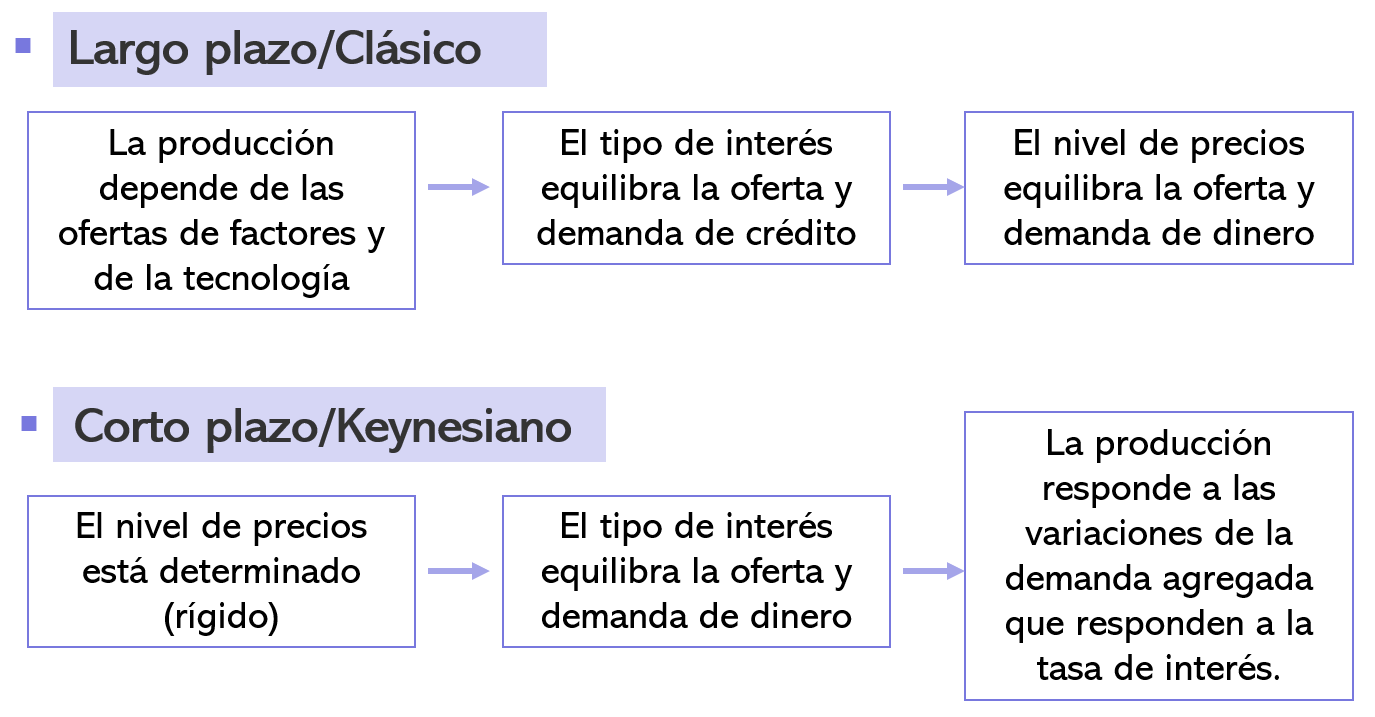
\includegraphics[width=11cm]{Figures/P18.png}\

\end{frame}


\begin{frame}{El enfoque Clásico y Keynesiano: Oferta Agregada}

\begin{itemize}
        \footnotesize\item La curva OA relaciona P (precios) con Y (producto).
        \footnotesize\item La forma de esta curva determina el mercado de trabajo.
\end{itemize}
\vspace{3mm}
\centering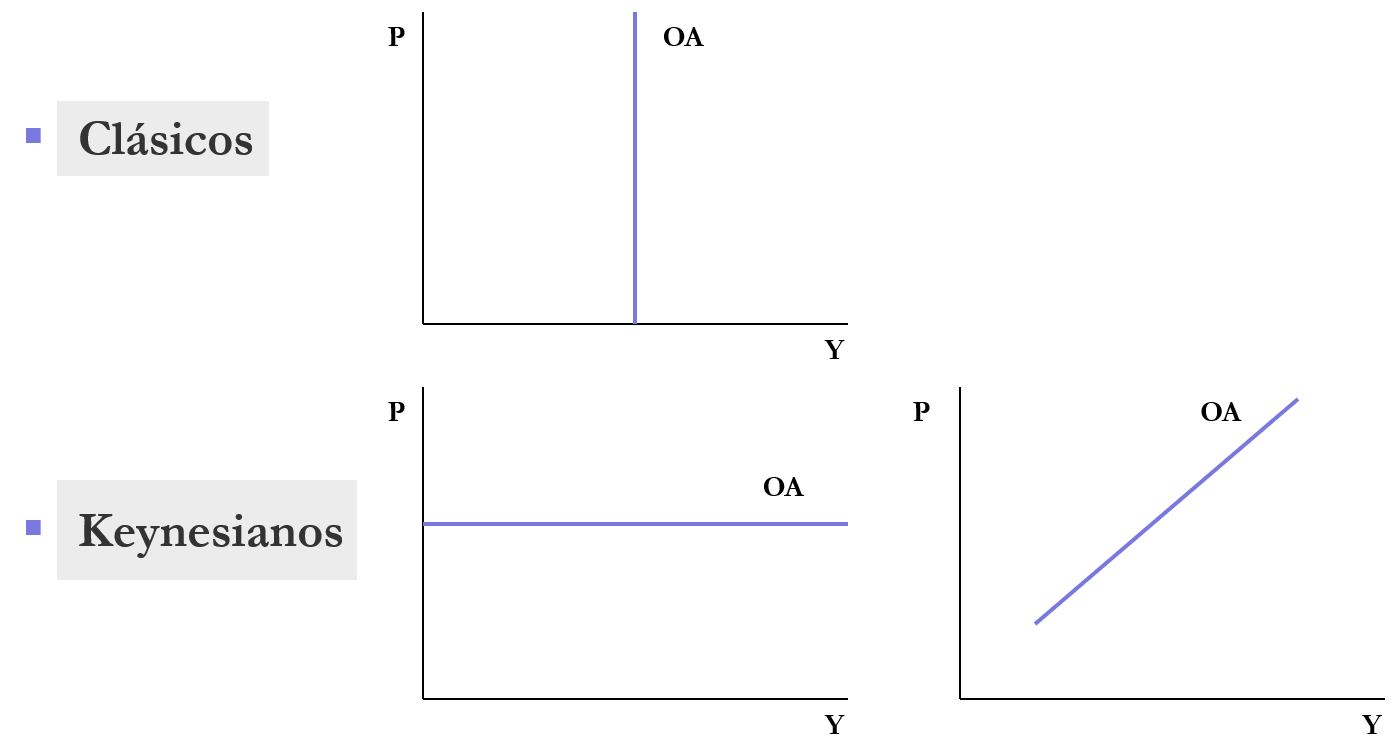
\includegraphics[width=10.5cm]{Figures/P19.png}\

\end{frame}


\begin{frame}{El enfoque Clásico y Keynesiano: Demanda Agregada}

\centering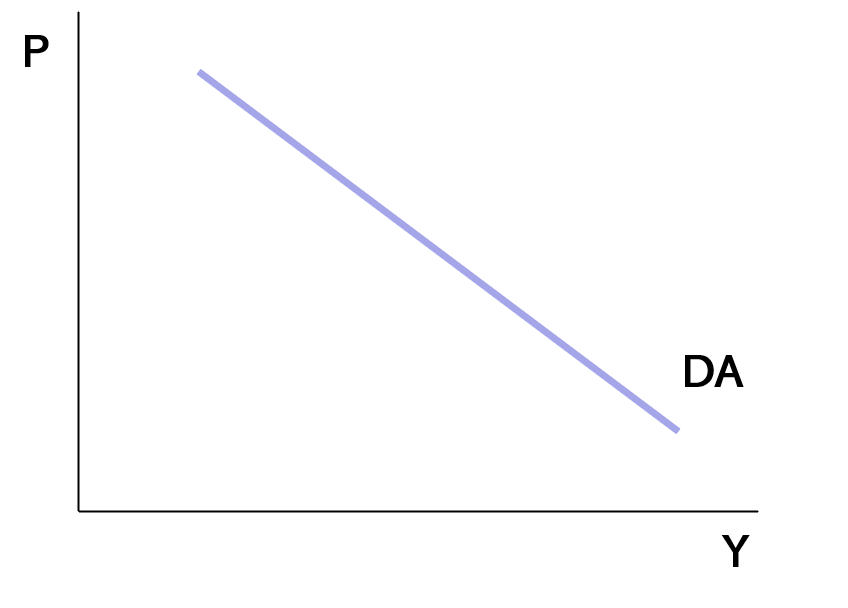
\includegraphics[width=6cm]{Figures/P20.png}\

    \begin{itemize}
        \item La forma de esta curva determina como C (consumo) e I (inversión) reaccionan frente al nivel de P (precios)
        \item El consumo y la inversión caen debido al incremento en los precios:
            \begin{itemize}
                \item Efecto riqueza
                \item Efecto tasa de interés: un aumento de P sin cambiar M lleva a tasas de interés más altas que hacen caer C e I.
            \end{itemize}
    \end{itemize}

\end{frame}



\begin{frame}{Shocks a la Demanda Agregada}
    
\centering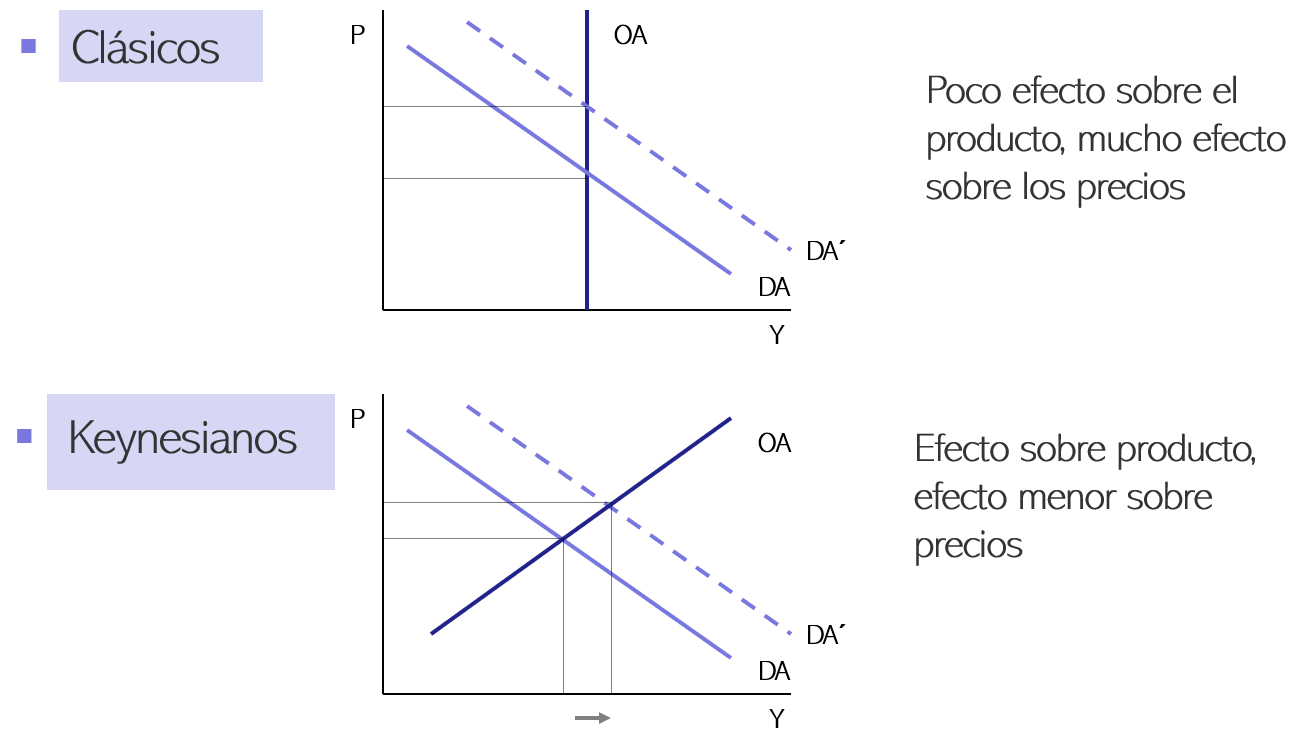
\includegraphics[width=11cm]{Figures/P21.png}\
    
\end{frame}


\begin{frame}{Shocks a la Oferta Agregada}

Los shocks de oferta negativos  producen un fenómeno que se conoce como estanflación

\begin{figure} [H]
\centering
\begin{minipage}{.5\textwidth}
  \centering
  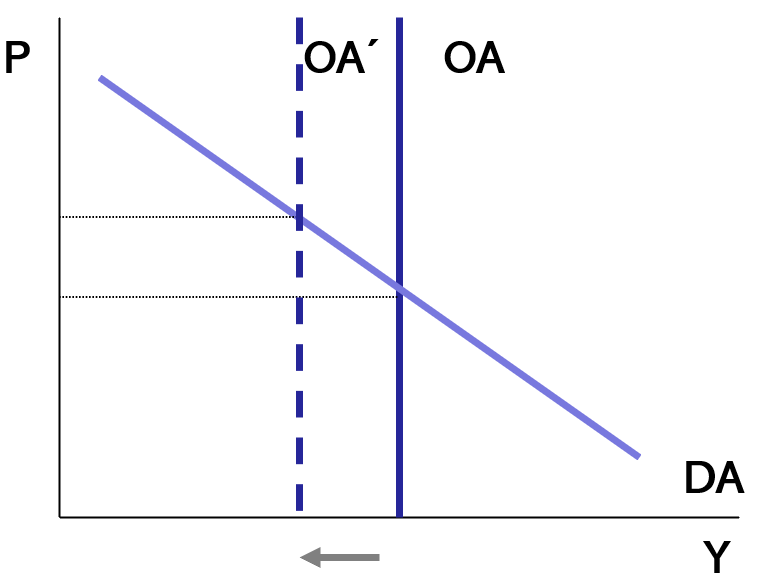
\includegraphics[width=0.9\textwidth]{Figures/P22_1.png}
  \caption{\textbf{Clásicos}}
  \label{a}
\end{minipage}%
\begin{minipage}{.5\textwidth}
  \centering
  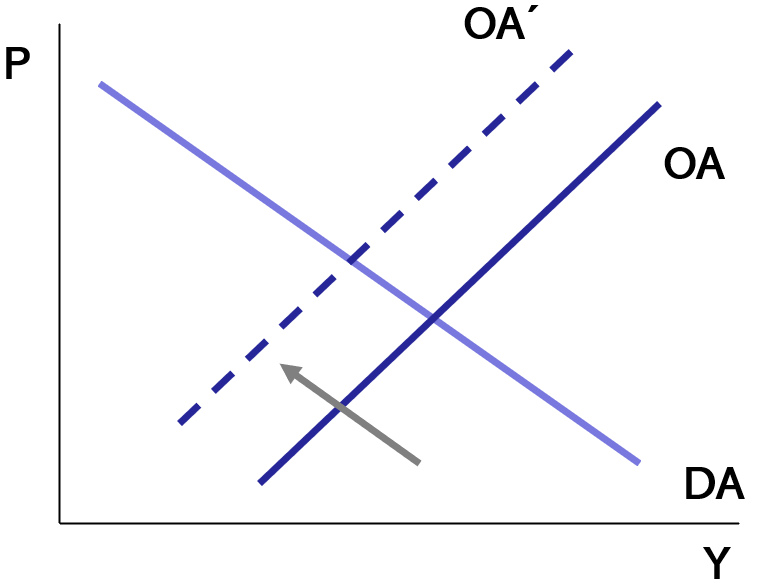
\includegraphics[width=0.9\textwidth]{Figures/P22_2.png}
  \caption{\textbf{Keynesianos}}
  \label{b}
\end{minipage}
\\
\end{figure}

\end{frame}


\begin{frame}{Ciclos: los Clásicos}

\begin{itemize}
    \item La explicación clásica de las fluctuaciones viene por cambios en la oferta agregada
\end{itemize}

\vspace{2mm}

\centering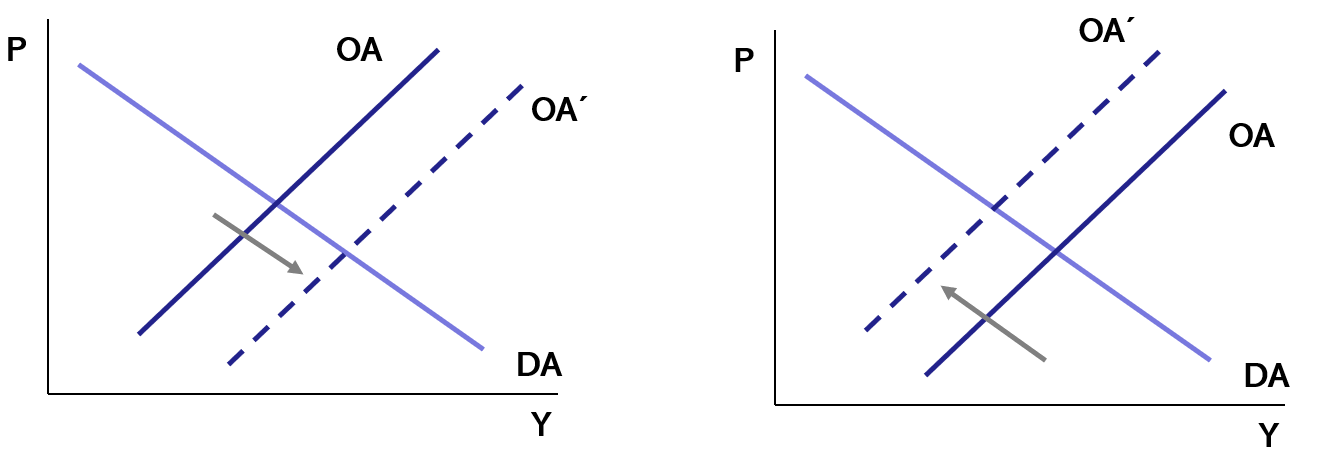
\includegraphics[width=11cm]{Figures/P23.png}\

\end{frame}



\begin{frame}{ Ciclos: los Keynesianos}

\begin{itemize}
    \item La explicación keynesiana de las fluctuaciones viene por cambios en la demanda agregada
\end{itemize}

\vspace{2mm}

\centering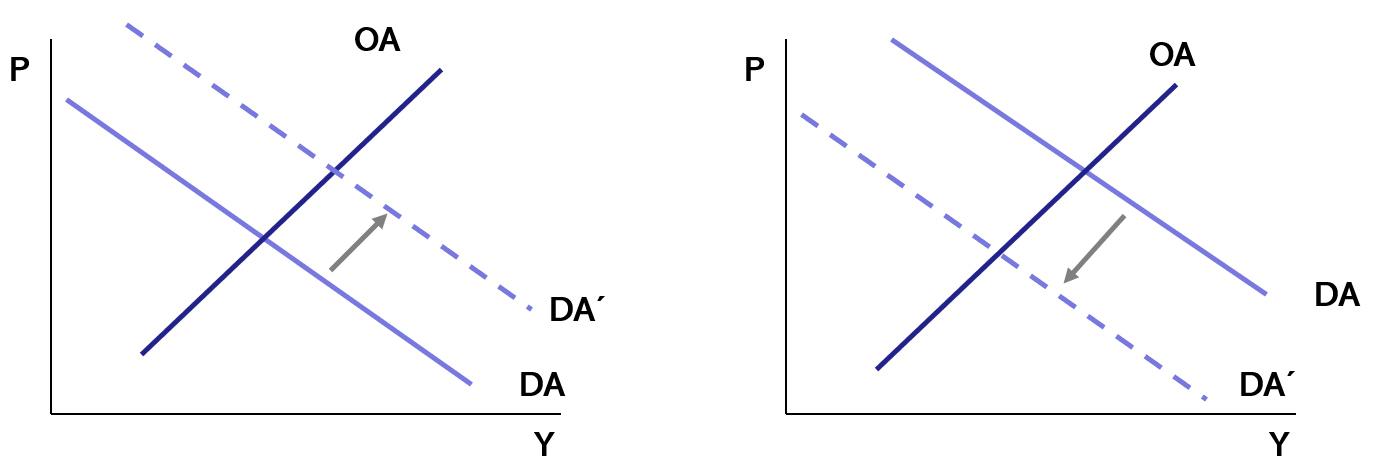
\includegraphics[width=12cm]{Figures/P24.png}\

\end{frame}

%---------------------------------------------------------------------------%
%---------------------------------------------------------------------------%

%\begin{frame}{}
%\centering 	\huge \textbf{El mercado de trabajo y la oferta %agregada} 
%\vspace{2mm}
%\hrule
%\end{frame}
%---------------------------------------------------------------------------%
%---------------------------------------------------------------------------%

%---------------------------------------------------------------------------%









\begin{frame}{ Mercado de trabajo: definiciones}
\begin{itemize}
    \item ¿Quiénes ofrecen trabajo?
    \vspace{2mm}
    \item ¿Quiénes demandan trabajo?
\end{itemize} 
\end{frame}


\begin{frame}{Mercado de trabajo: demanda de trabajo}
\begin{itemize}
\item Depende de los precios y de la productividad 
\end{itemize}
\centering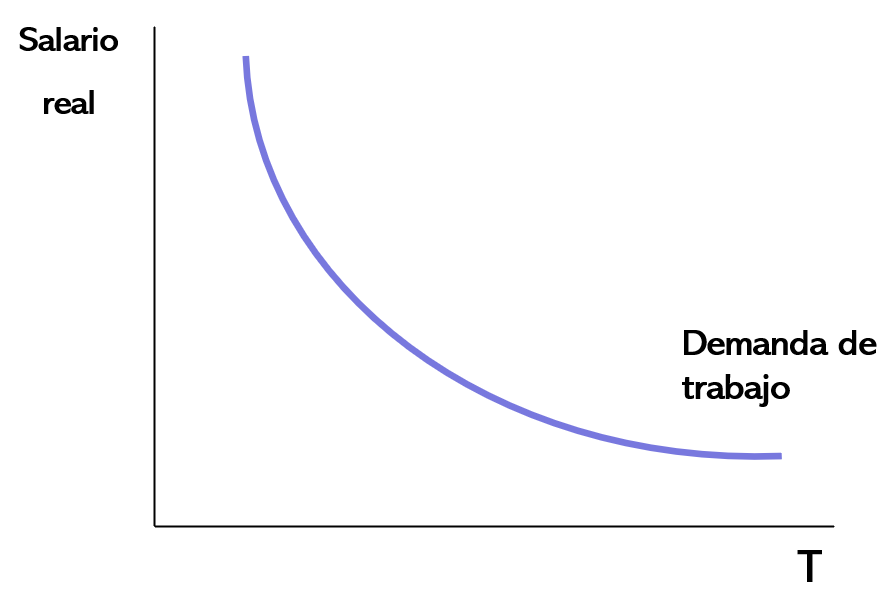
\includegraphics[width=9cm]{Figures/P27.png}\
\end{frame}


\begin{frame}{Mercado de trabajo: oferta de trabajo}

\begin{itemize}
    \item ¿ Cómo responde la oferta de trabajo ante un cambio en los salarios?
    \vspace{2mm}
    \begin{itemize}
    \item Shock temporario $\Rightarrow$ la oferta de trabajo aumenta \vspace{1mm}
    \item Shock permanente $\Rightarrow$ la oferta de trabajo no se modifica (mucho) \vspace{1mm}
   \item Un ejemplo que ilustra esto último: desde la época medieval hemos trabajado aprox unas 8 horas por día
    \end{itemize}
\end{itemize}
\end{frame}

\begin{frame}{Mercado de trabajo: el equilibrio}
\begin{itemize}
    \item Si el salario está por encima de su valor de equilibrio (salario real*) habrá desempleo
\end{itemize}

\begin{center}
\begin{figure}[H]
\renewcommand{\figurename}{Figure}
\begin{center}
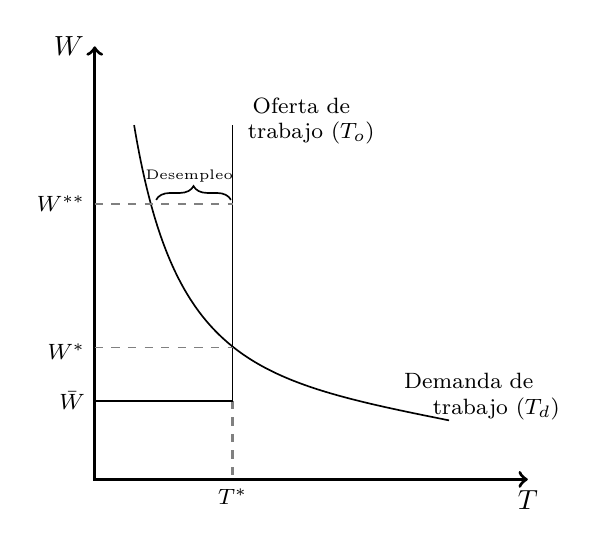
\begin{tikzpicture}[scale=0.5]
\draw[very thick,<->] (0,11) node[left]{$W$}--(0,0)--(11,0) node[below]{$T$};
\draw[semithick] (1,9).. controls (2,3) and (4, 2.5) .. (9, 1.5);
\node [] at (9.5,2.5) {\footnotesize Demanda de};
\node [] at (10.2,1.8) {\footnotesize trabajo ($T_d$)};
\draw[semithick](3.5,2)--(3.5,9);
\draw[thick, dashed, gray] (3.5,2)--(3.5,0);
\node [] at (5.25,9.5) {\footnotesize Oferta de};
\node [] at (5.5,8.8) {\footnotesize  trabajo ($T_o$)};
\node [below] at (3.5,0) {\footnotesize  $T^*$};
\node [left] at (0,3.25) {\footnotesize  $W^*$};
\draw[semithick, dashed,gray] (0,3.35)--(3.5,3.35);
\node [left] at (0,7) {\footnotesize  $W^{**}$};
\draw[semithick, dashed,gray] (0,7)--(3.5,7);
\draw (2.4,7.7) node[]{\tiny Desempleo};
\draw [semithick,decorate,decoration={brace,amplitude=5pt},xshift=-4pt,yshift=0pt](1.7,7.1) -- (3.6,7.1);
\node [left] at (0,2) {\footnotesize  $\bar{W}$}  ;
\draw[semithick] (0,2)--(3.5,2);
%\node [left] at (8,6) {\scriptsize  Keynesiano}  ;
%\node [left] at (7,4) {\scriptsize  Clásico}  ;
%\draw[semithick, <-] (3.75,6.75)--(4.5,6);
%\draw[semithick, <-] (3.75,3.45)--(4.65,4);
\end{tikzpicture}
\end{center}
\label{fig:C30.5}
\end{figure}
\end{center}  
\end{frame}


\begin{frame}{La visión de los Clásicos}
\begin{itemize}
    \item Según esta visión el mercado de trabajo siempre está en equilibrio:
    \vspace{2mm}
    \begin{itemize}
    \scriptsize\item Es decir que el salario real* es el de equilibrio
    \scriptsize\item De esta manera, el nivel de actividad es siempre el de pleno empleo
    \scriptsize \item Y la oferta agregada es vertical
    \end{itemize}
\end{itemize}
\centering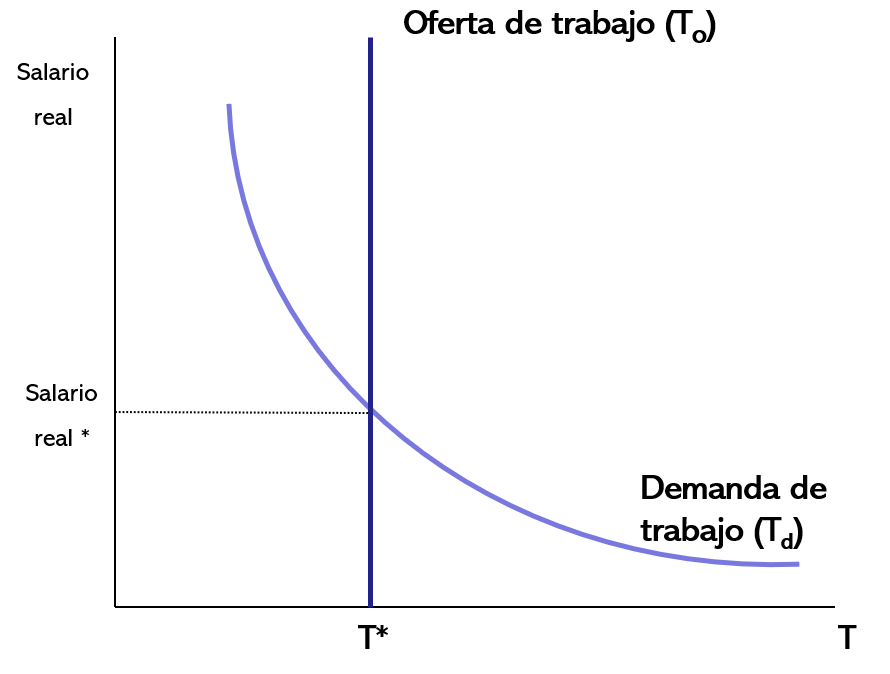
\includegraphics[width=8cm]{Figures/P29.png}\
\end{frame}


\begin{frame}{¿Y el desempleo?}
    \centering
\includegraphics[width=5cm]{Figures/P29b.png}\
\begin{itemize}
\item Desempleo Friccional
\item Salarios de reserva altos
\item Problemas de medición
\end{itemize}
\end{frame}


\begin{frame}{La visión Keynesiana}
\begin{itemize}
    \footnotesize\item El mercado de trabajo \textbf{no siempre} está en equilibrio:
    \vspace{2mm}
    \begin{itemize}
    \scriptsize\item ¿Por qué puede el salario real permanecer fuera del equilibrio?
    \begin{itemize}
        \scriptsize\item Rigideces nominales
        \scriptsize\item Sindicatos
        \scriptsize\item Contratos de largo plazo
        \scriptsize\item Salarios de eficiencia
       \end{itemize}
    \end{itemize}
\end{itemize}
    \centering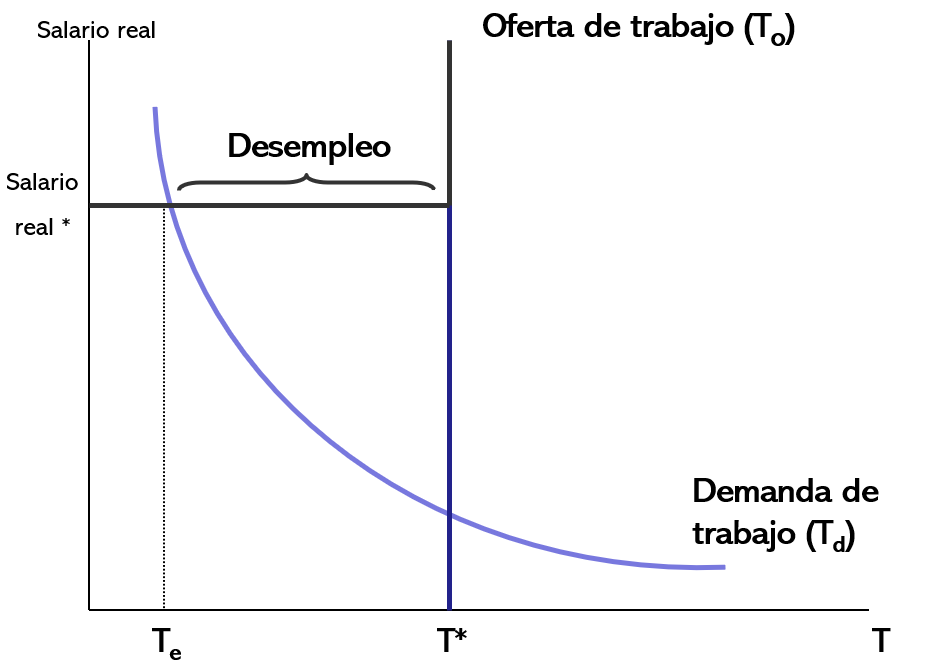
\includegraphics[width=8cm]{Figures/P30.png}\
\end{frame}


\begin{frame}{La visión Keynesiana}
\begin{itemize}
\item Un aumento en la demanda por trabajo aumenta el nivel de actividad con un efecto reducido en salarios y precios.
\item La oferta agregada se transforma, entonces, en horizontal
\end{itemize}
    \centering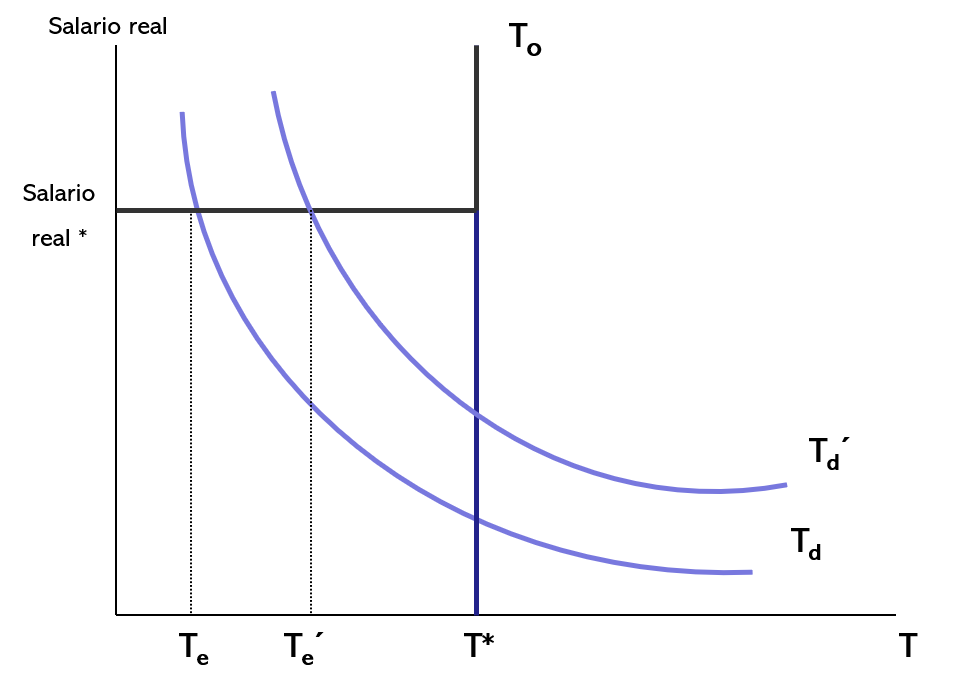
\includegraphics[width=8cm]{Figures/P31.png}\
\end{frame}



\begin{frame}{¿Qué es el desempleo y cómo se mide?}
\begin{itemize}
    \item Desempleo involuntario: es el desempleo de la gente que busca pero no encuentra empleo
    \item Fuerza laboral: PEA (Población Económicamente Activa)
        \begin{itemize}
            \item Empleados
            \item Desempleados
        \end{itemize}
\end{itemize}
\vspace{3mm}
\centering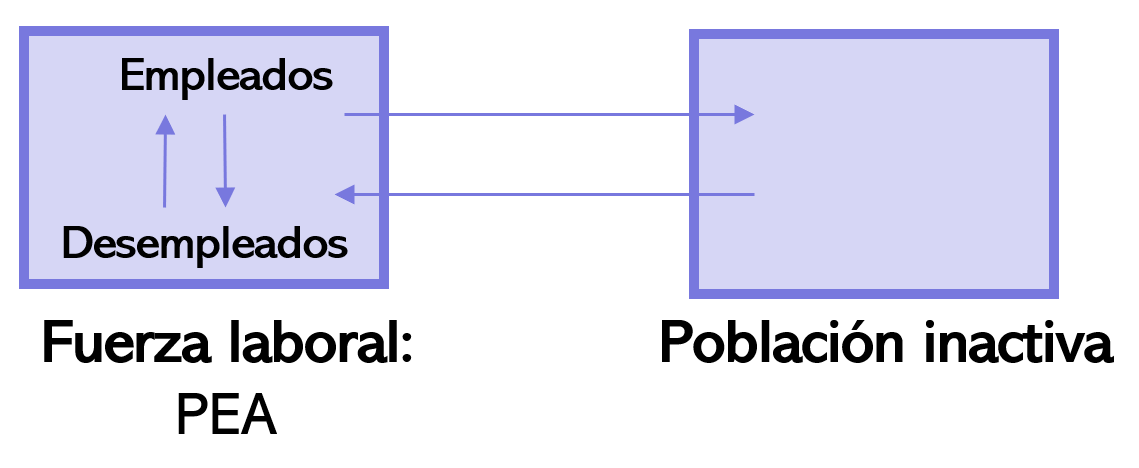
\includegraphics[width=6cm]{Figures/P32.png}\
\end{frame}

\begin{frame}{Indicadores básicos del mercado laboral}
\begin{itemize}
    \item Tasa de desempleo: $\frac{\text {Número de desempleados}}{\text{PEA}}$
    \vspace{3mm}
    
        \dangersignw Puede variar por: 
        \begin{itemize}
            \vspace{2mm}
        \item Cambios en el número de desempleados
            \vspace{2mm}
        \item Cambios en la fuerza laboral (PEA)
        \end{itemize}
           \vspace{3mm}
    \item Tasa de empleo: $\frac{\text {Número de empleados}}{\text{Población}}$
    \vspace{3mm}
    \item Tasa de participación: $\frac{\text {PEA}}{\text{Población}}$
\end{itemize}
\end{frame}

\begin{frame}{La tasa de desempleo en Argentina}
\centering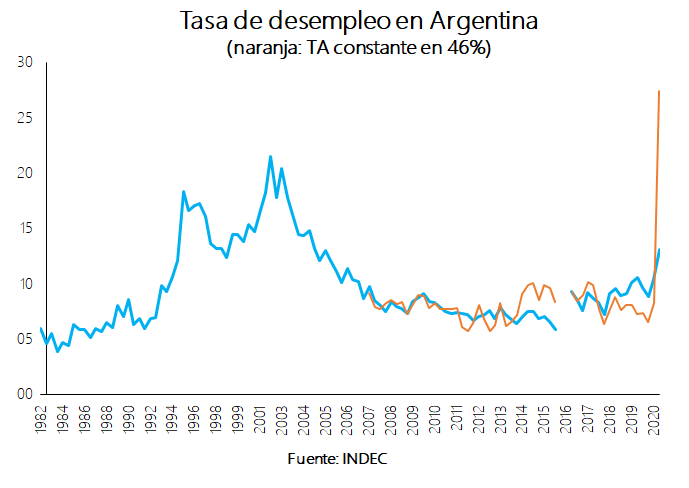
\includegraphics[width=11cm]{Figures/P34.png}
\end{frame}

\begin{frame}{Problemas con la serie de desempleo de INDEC}
\centering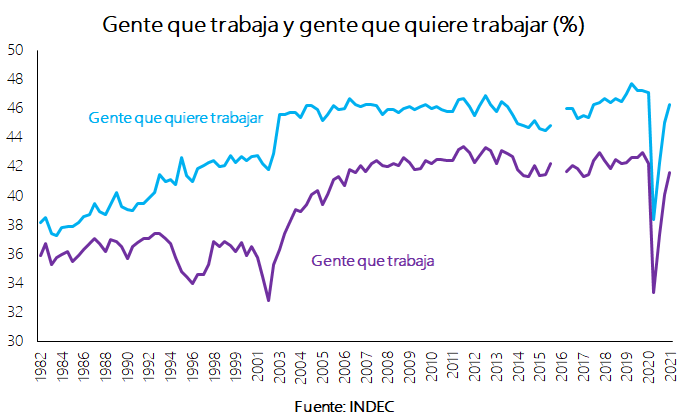
\includegraphics[width=11cm]{Figures/C30.15b.png}
\end{frame}

\begin{frame}{El mercado de trabajo en la Argentina (1)}
\centering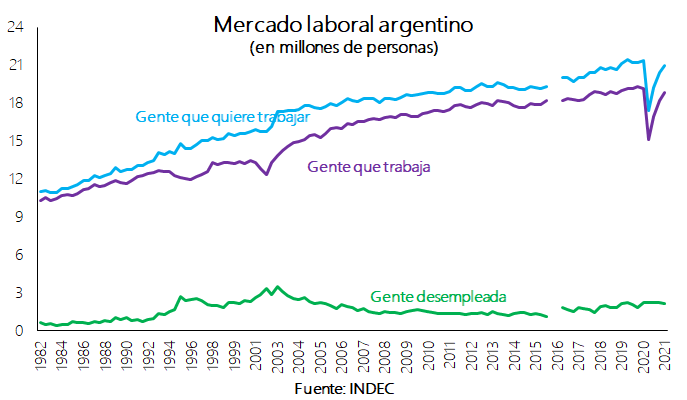
\includegraphics[width=11cm]{Figures/C30.16b.png}
\end{frame}

\begin{frame}{El mercado de trabajo en la Argentina (2)}
\centering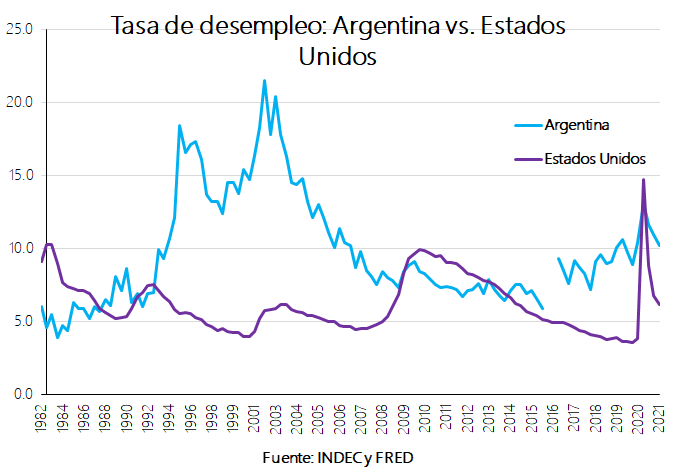
\includegraphics[width=11cm]{Figures/C30.17b.png}
\end{frame}

\begin{frame}{La recuperación de EE.UU. tardó en ocupar trabajo}
\centering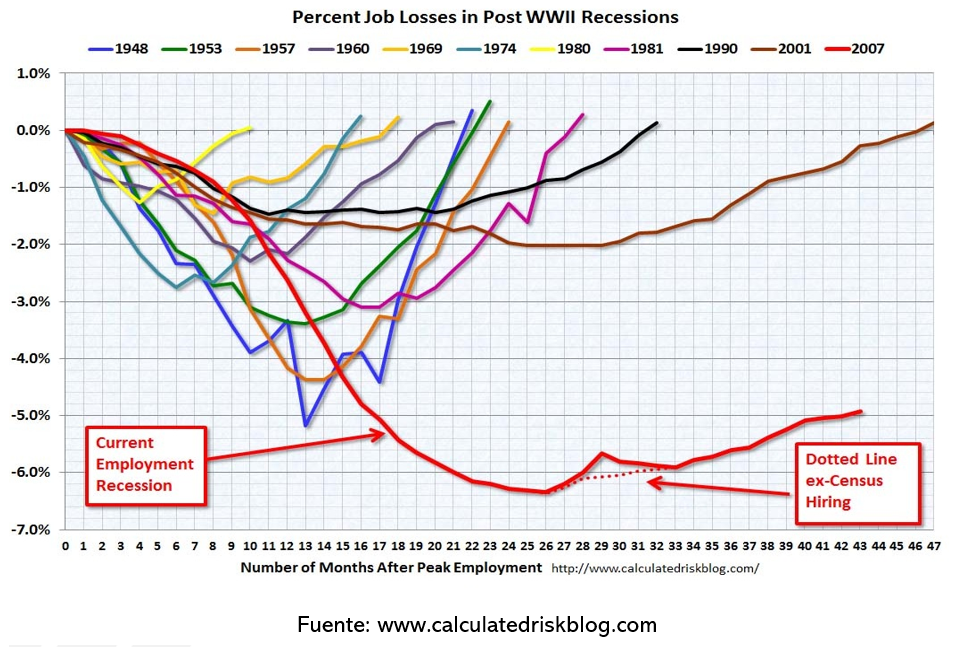
\includegraphics[width=12cm]{Figures/P39.png}\
\end{frame}


\begin{frame}{La recuperación de Argentina}
\centering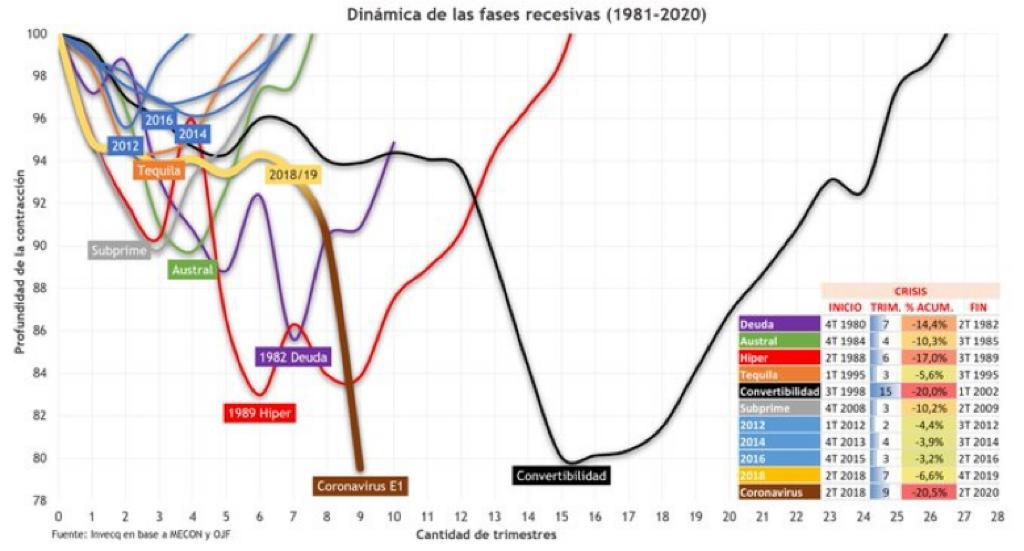
\includegraphics[width=11cm]{Recesiones.jpg}\
\end{frame}


\begin{frame}{¿Por qué vamos a estudiar el mercado de crédito?}
    \begin{itemize}
        \item Queremos analizar la voluntad de consumir e invertir de los agentes económicos \vspace{1mm}
        \begin{itemize}
            \item Porque analizar estas dos variables es central para la determinación del consumo y la inversión y, de la demanda agregada
            \item ¿Qué era la demanda agregada? 
        \end{itemize}
        \vspace{3mm}
        \item El mercado de crédito asigna los ahorros de la sociedad a la inversión \vspace{1mm}
        \begin{itemize}
            \item Este mercado representa el mecanismo por el cual la economía reparte la demanda agregada entre consumo e inversión
        \end{itemize}
    \end{itemize}
\end{frame}

\begin{frame}{La Demanda Agregada}
\begin{itemize}
\begin{tcolorbox}[width=4in,
                  interior hidden,
                  boxsep=0pt,
                  left=0pt,
                  right=0pt,
                  top=2pt,
                  ]%%
$$ Y = C + I + G $$
\end{tcolorbox}
    \end{itemize}
\centering donde C + I + G es la absorción.
\vspace{1cm}
\begin{itemize}
        \item \textbf{C} depende de las expectativas, el ingreso disponible e impuestos
        \item \textbf{I} depende de las expectativas, impuestos y productividad
        \item Las dos se ven afectadas por la tasa de interés
        \item Noten que estamos en una economía sin sector externo (no hay exportaciones ni importaciones)
\end{itemize}
\end{frame}

\begin{frame}{¿Cómo se determina el consumo?}
    \begin{itemize}
        \item Depende del ingreso actual y el esperado
        \item La teoría básica del consumo es la de la “suavización del consumo” a lo largo de la vida
        \item Lo que implica que 
            \begin{itemize}
            \item Ante cambios temporarios en el ingreso
                \begin{itemize}
                \item hay pequeños cambios en el consumo (y mucho cambio en el ahorro)
                \end{itemize}            
            \item Ante cambios permanentes en el ingreso
                \begin{itemize}
                \item hay grandes cambios en el consumo actual (y poco cambio en el ahorro)
                \end{itemize}
            \end{itemize}
        \item El consumo cambia más ante cambios en las expectativas que ante cambios reales!!!
        \item Pero la tasa de interés también lo afecta alterando el deseo de "consumo hoy" versus "consumo mañana"
    \end{itemize}
\end{frame}


\begin{frame}{Shocks de ingreso permanentes y transitorios}

\begin{center}
\begin{figure}[h!]
\renewcommand{\figurename}{Figure}
\begin{center}
    \begin{minipage}[b]{0.45\textwidth}
        \begin{center}
\begin{tikzpicture}[scale=0.4]
\draw[very thick,<->] (0,11) node[left]{$C,Y$}--(0,0)--(11,0) node[below]{$t$};

\draw[semithick, gray](0, 4)--(3, 4)--(3,6)--(8.5,6) node[right] {\scriptsize $Y=C$};
\draw[thick, dashed, red](0, 4)--(3, 4)--(3,6)--(8.5,6);
\draw[thick, dotted](3,4)--(3,0) node [below] {\footnotesize $t_0$};
\end{tikzpicture}
\end{center}
     \end{minipage}
  %  \hfill
    \begin{minipage}[b]{0.45\textwidth}
    \begin{center}
\begin{tikzpicture}[scale=0.4]
\draw[very thick,<->] (0,11) node[left]{$C,Y$}--(0,0)--(11,0) node[below]{$t$};
\draw[semithick, gray](0, 4)--(3, 4)--(3,6)--(5,6)--(5,4)--(8.5,4)node[right] {\scriptsize $Y$};
\draw[thick, dashed, red](0, 4)--(3, 4)--(3,5)--(8.5,5) node[right] {\scriptsize $C$};
\draw[thick, dotted](3,4)--(3,0) node [below] {\footnotesize $t_0$};
%\draw[thick, dashed](0, 4)--(3,4)--(3,6)--(5,6);
\end{tikzpicture}
\end{center}
    \end{minipage}
\end{center}
\end{figure}
\end{center}
\end{frame}


\begin{frame}{Modelo de elección del consumo presente y consumo futuro: la restricción presupuestaria}
    \begin{center}
\begin{figure}[H]
\renewcommand{\figurename}{Figure}
\begin{center}
\begin{tikzpicture}[scale=0.5]
\draw[very thick,<->] (0,11) node[left]{$c_{t+1}$}--(0,0)--(11,0) node[below]{$c_{t}$};
\draw[semithick] (0,7)--(8,0);
 \draw[thick,gray, dashed](3.5, 3.95)--(3.5, 0);
  \draw[thick,gray, dashed](3.5, 3.95)--(0, 3.95);
 \node[below] at (3.5,0) {\footnotesize $y_t$};
  \node[left] at (0,3.95) {\footnotesize $y_{t+1}$};
  \draw[fill] (3.5,3.95) circle [radius =0.11] ;
\end{tikzpicture}
\end{center}
\end{figure}
\end{center} 
\end{frame}


\begin{frame}{Modelo de elección del consumo presente y consumo futuro: la curva de indiferencia}
\begin{center}
\begin{figure}[H]
\renewcommand{\figurename}{Figure}
\begin{center}
\begin{tikzpicture}[scale=0.5]
\draw[very thick,<->] (0,11) node[left]{$c_{t+1}$}--(0,0)--(11,0) node[below]{$c_{t}$};
%\draw[semithick] (2,8).. controls (2.5,2.5) and (4,1) ..(8,0);
\draw[semithick] (2,8).. controls (2.5,2.5) and (4,0.75) ..(8.25,0.65);
 \draw[thick,gray, dashed](2.15, 7)--(2.85, 4);
   \draw[fill] (2.1,7) circle [radius =0.11] ;
 \draw[thick,gray, dashed](4.2, 1.9)--(2.85, 4);      
      \draw[fill] (2.8,3.95) circle [radius =0.11] ;
\draw[fill] (4.2,1.8) circle [radius =0.11] ;      
\draw[semithick, ->] (2.1,7)--(2.1,4);
\draw[semithick, ->] (2.1,3.95)--(2.7,3.95);
\draw[semithick, ->] (2.8,3.95)--(2.8,1.8);
\draw[semithick, ->] (2.85,1.8)--(4,1.8);
\end{tikzpicture}
\end{center}
\end{figure}
\end{center}  
\end{frame}

\begin{frame}{ Modelo de elección del consumo presente y consumo futuro: el equilibrio}
\begin{center}
\begin{figure}[H]
\renewcommand{\figurename}{Figure}
\begin{center}
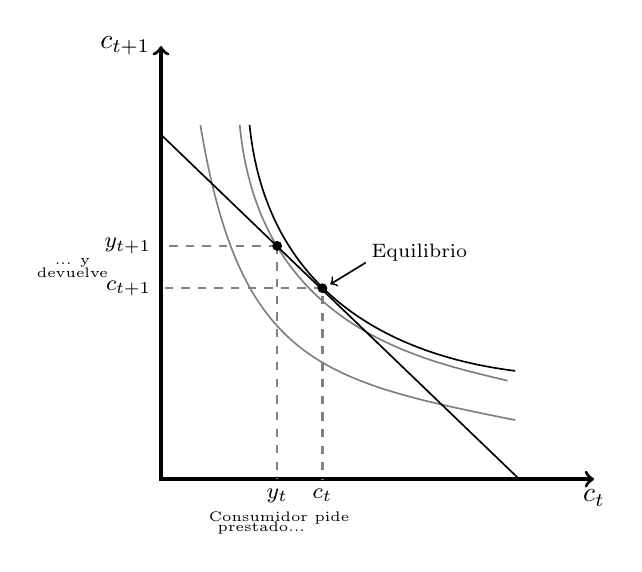
\begin{tikzpicture}[scale=0.5]
\draw[very thick,<->] (0,11) node[left]{$c_{t+1}$}--(0,0)--(11,0) node[below]{$c_{t}$};
\draw[semithick, gray] (1,9).. controls (2,3) and (4, 2.5) .. (9, 1.5) ;
\draw[semithick, gray] (2,9).. controls (2.5,3.75) and (6.8, 3) .. (8.8, 2.5);
\draw[semithick] (2.25,9).. controls (2.75,4) and (7, 3) .. (9, 2.75);
\draw[semithick] (0,8.75)--(9.1,0);
 \draw[thick,gray, dashed](4.1, 4.65)--(4.1, 0);
 \draw[thick,gray, dashed](4.1, 4.85)--(0, 4.85);
 \draw[fill] (4.1,4.85) circle [radius =0.11] ;  
 \node[below] at (4.1,0) {\footnotesize $c_t$};
 \node[left] at (0,4.85){\footnotesize $c_{t+1}$};
 \draw[thick,gray, dashed](2.95, 5.925)--(2.95, 0);
 \draw[thick,gray, dashed](2.95, 5.925)--(0, 5.925);
 \draw[fill] (2.95,5.925) circle [radius =0.11] ;   
 \node[below] at (2.95,0) {\footnotesize $y_t$};
 \node[left] at (0,5.925){\footnotesize $y_{t+1}$};
 \node [right] at (5.1,5.75) {\scriptsize  Equilibrio}  ;
\draw[semithick, <-] (4.3,4.95)--(5.2,5.5);
%\draw [semithick,decorate,decoration={brace,amplitude=3pt,mirror},xshift=5pt,yshift=0pt](2.75,-0.6) -- (3.9,-0.6);
\draw (3,-1) node[]{\tiny Consumidor pide};
\draw (2.55,-1.25) node[]{\tiny prestado...};
%\draw [semithick,decorate,decoration={brace,amplitude=3pt,mirror},xshift=0pt,yshift=5pt](-1.25,5.85) -- (-1.25,4.7);
\draw (-2.25,5.5) node[]{\tiny ... y};
\draw (-2.25,5.25) node[]{\tiny devuelve};
\end{tikzpicture}
\end{center}
\end{figure}
\end{center}  
\end{frame}


\begin{frame}{El efecto de un cambio en la tasa de interés}
\begin{center}
\begin{figure}[H]
\renewcommand{\figurename}{Figure}
\begin{center}
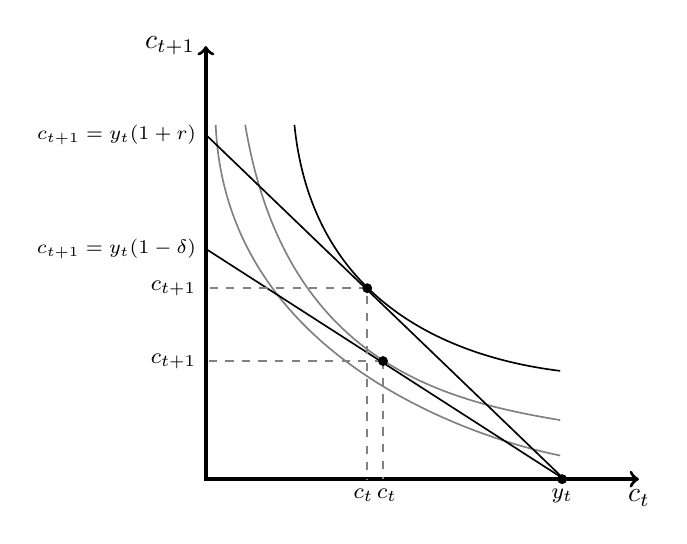
\begin{tikzpicture}[scale=0.5]
\draw[very thick,<->] (0,11) node[left]{$c_{t+1}$}--(0,0)--(11,0) node[below]{$c_{t}$};
\draw[semithick, gray] (1,9).. controls (2,3) and (6, 2) .. (9, 1.5) ;
%\draw[semithick, gray] (0.25,9).. controls (0.5,3) and (7, 1) .. (9, 0);
\draw[semithick, gray] (0.25,9).. controls (0.5,3) and (7, 1) .. (9, 0.6);
\draw[semithick] (2.25,9).. controls (2.75,4) and (7, 3) .. (9, 2.75);
\draw[semithick] (0,8.75)--(9.1,0);
\draw[semithick] (0,5.85)--(9.1,0);
  \draw[thick,gray, dashed](4.1, 4.65)--(4.1, 0);
  \draw[thick,gray, dashed](4.1, 4.85)--(0, 4.85);
  \draw[fill] (4.1,4.85) circle [radius =0.11] ;  
  \node[below] at (4,0) {\footnotesize $c_t$};
  \node[left] at (0,4.85){\footnotesize $c_{t+1}$};
%  \draw[thick,gray, dashed](2.95, 5.925)--(2.95, 0);
%  \draw[thick,gray, dashed](2.95, 5.925)--(0, 5.925);
  \draw[thick,gray, dashed](4.5, 3)--(4.5, 0);
  \draw[thick,gray, dashed](4.5, 3)--(0, 3);
  \node[below] at (4.6,0) {\footnotesize $c_t$};
  \node[left] at (0,3){\footnotesize $c_{t+1}$};
  \draw[fill] (4.5,3) circle [radius =0.11] ;   
    \draw[fill] (9.05,0) circle [radius =0.11] node [below] {\footnotesize $y_t$} ;   
  \node[left] at (0,5.85){\scriptsize $c_{t+1} = y_t (1-\delta)$};   
  \node[left] at (0,8.75){\scriptsize $c_{t+1} = y_t (1+r)$};
\end{tikzpicture}
\end{center}
\end{figure}
\end{center}  
\end{frame}

\begin{frame}{Apalancamiento}
   \begin{center}
\begin{figure}[H]
\renewcommand{\figurename}{Figure}
\begin{center}
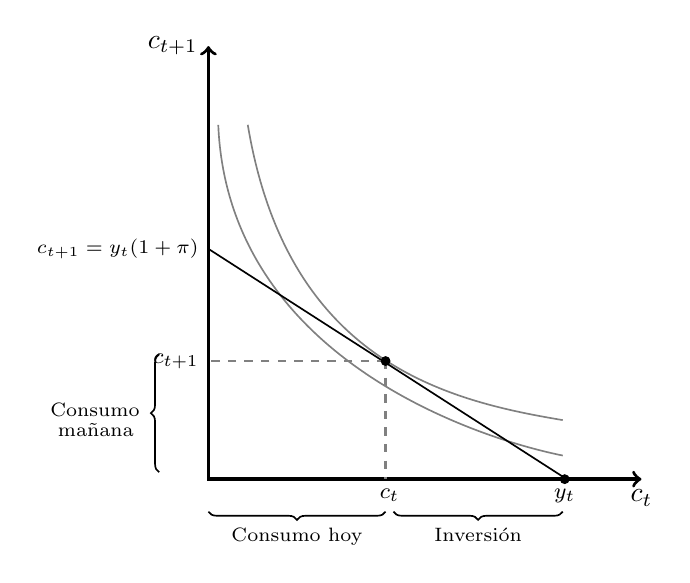
\begin{tikzpicture}[scale=0.5]
\draw[very thick,<->] (0,11) node[left]{$c_{t+1}$}--(0,0)--(11,0) node[below]{$c_{t}$};
\draw[semithick, gray] (1,9).. controls (2,3) and (6, 2) .. (9, 1.5) ;
%\draw[semithick, gray] (0.25,9).. controls (0.5,3) and (7, 1) .. (9, 0);
\draw[semithick, gray] (0.25,9).. controls (0.5,3) and (7, 1) .. (9, 0.6);
\draw[semithick] (0,5.85)--(9.1,0);
  \draw[thick,gray, dashed](4.5, 3)--(4.5, 0);
  \draw[thick,gray, dashed](4.5, 3)--(0, 3);
  \node[below] at (4.6,0) {\footnotesize $c_t$};
  \node[left] at (0,3){\footnotesize $c_{t+1}$};
  \draw[fill] (4.5,3) circle [radius =0.11] ;   
    \draw[fill] (9.05,0) circle [radius =0.11] node [below] {\footnotesize $y_t$} ;   
  \node[left] at (0,5.85){\scriptsize $c_{t+1} = y_t (1+\pi)$};   
 \draw [semithick,decorate,decoration={brace,amplitude=3pt},xshift=0pt,yshift=5pt](-1.25,0) -- (-1.25,3);  
  \draw [semithick,decorate,decoration={brace,amplitude=3pt, mirror},xshift=0pt,yshift=5pt](0,-1) -- (4.5,-1); 
  
    \draw [semithick,decorate,decoration={brace,amplitude=3pt, mirror},xshift=0pt,yshift=5pt](4.7,-1) -- (9,-1); 
  \node[left] at (-1.5,1.75){\scriptsize Consumo};   
    \node[left] at (-1.65,1.25){\scriptsize mañana};
  \node[below] at (2.25,-1){\scriptsize Consumo hoy};      
    \node[below] at (6.85,-1){\scriptsize Inversión};     
\end{tikzpicture}
\end{center}
\end{figure}
\end{center}   
\end{frame}


\begin{frame}{ Apalancamiento}
    \begin{center}
\begin{figure}[H]
\renewcommand{\figurename}{Figure}
\begin{center}
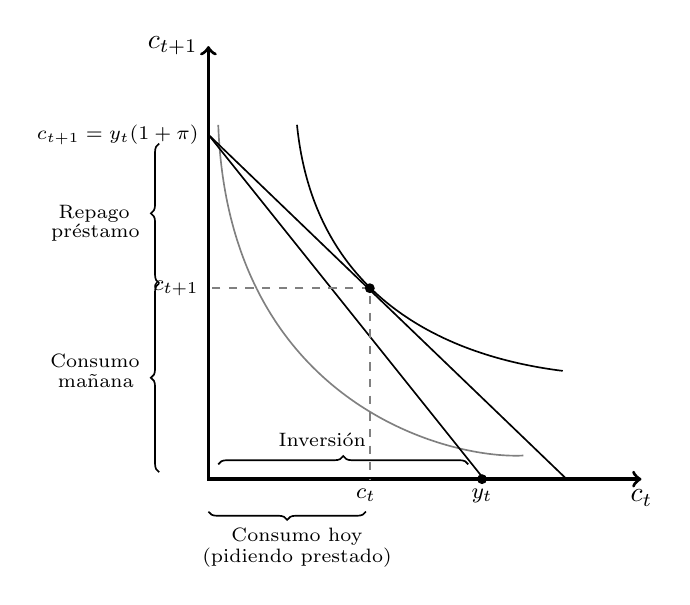
\begin{tikzpicture}[scale=0.5]
\draw[very thick,<->] (0,11) node[left]{$c_{t+1}$}--(0,0)--(11,0) node[below]{$c_{t}$};
%\draw[semithick, gray] (0.25,9).. controls (0.5,2) and (6, 0.5) .. (7, 0);
\draw[semithick, gray] (0.25,9).. controls (0.5,2) and (6, 0.5) .. (8, 0.6);
\draw[semithick] (2.25,9).. controls (2.75,4) and (7, 3) .. (9, 2.75);
\draw[semithick] (0,8.75)--(9.1,0);
\draw[semithick] (0,8.75)--(7,0);
  \draw[thick,gray, dashed](4.1, 4.65)--(4.1, 0);
  \draw[thick,gray, dashed](4.1, 4.85)--(0, 4.85);
  \draw[fill] (4.1,4.85) circle [radius =0.11] ;  
  \node[below] at (4,0) {\footnotesize $c_t$};
  \node[left] at (0,4.85){\footnotesize $c_{t+1}$};
    \draw[fill] (6.95,0) circle [radius =0.11] node [below] {\footnotesize $y_t$} ;   
  \node[left] at (0,8.75){\scriptsize $c_{t+1} = y_t (1+\pi)$}; 
   \draw [semithick,decorate,decoration={brace,amplitude=3pt},xshift=0pt,yshift=5pt](-1.25,0) -- (-1.25,4.8); 
      \draw [semithick,decorate,decoration={brace,amplitude=3pt,mirror},xshift=0pt,yshift=5pt](-1.25,8.35) -- (-1.25,4.8); 
  \draw [semithick,decorate,decoration={brace,amplitude=3pt, mirror},xshift=0pt,yshift=5pt](0,-1) -- (4,-1); 
\draw [semithick,decorate,decoration={brace,amplitude=3pt},xshift=0pt,yshift=5pt](0.25,0.2) -- (6.6,0.2); 
  \node[left] at (-1.5,3){\scriptsize Consumo};   
    \node[left] at (-1.65,2.5){\scriptsize mañana};
  \node[below] at (2.25,-1){\scriptsize Consumo hoy};
  \node[below] at (2.25,-1.5){\scriptsize (pidiendo prestado)};
    \node[left] at (4.25,1){\scriptsize Inversión};
      \node[left] at (-1.75,6.75){\scriptsize Repago };   
    \node[left] at (-1.5,6.25){\scriptsize préstamo};
\end{tikzpicture}
\end{center}
\end{figure}
\end{center} 
\end{frame}

\begin{frame}{El Gran Elon}
   \begin{figure} [H]
    \centering
    \href{https://twitter.com/Stelladmarco/status/1103059259586052097}{
    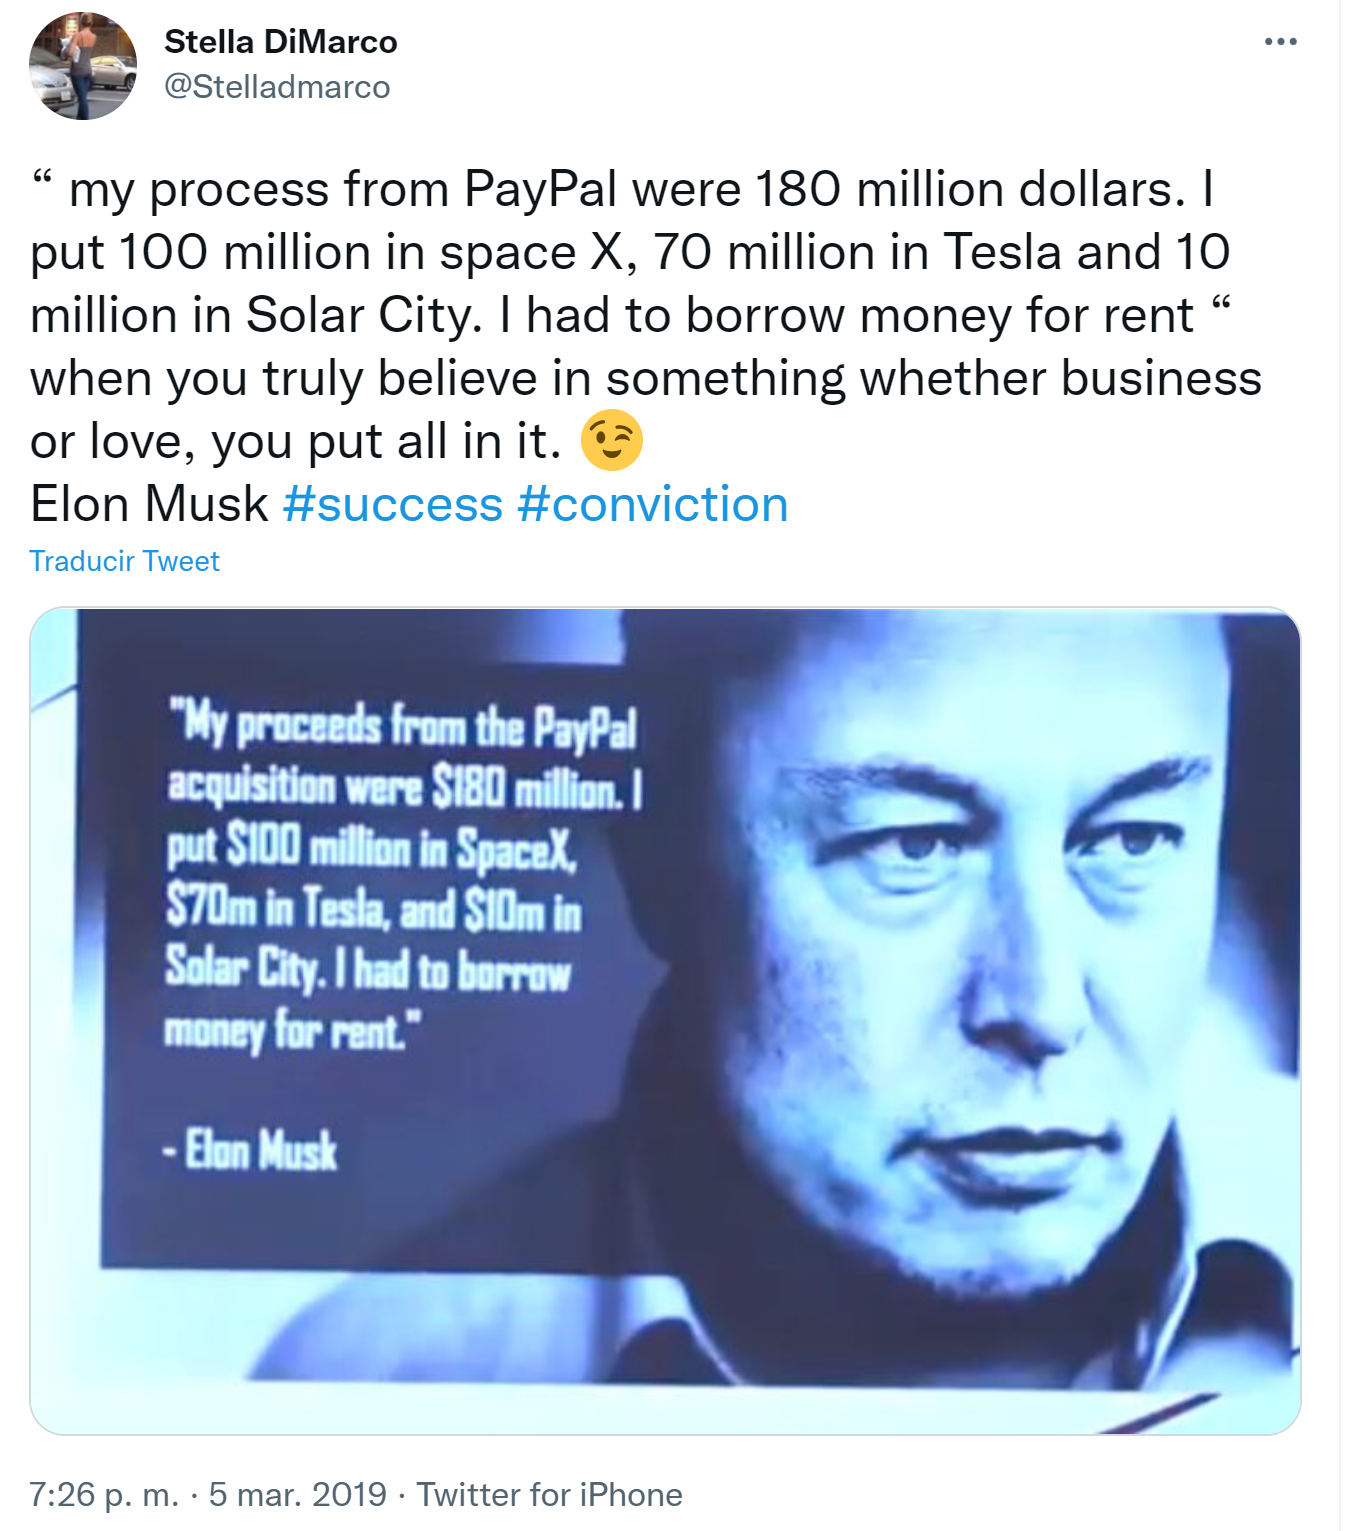
\includegraphics[scale=0.5]{Figures/C31.9.png}}
\end{figure} 
\end{frame} 


\begin{frame}{ Otras teorías del ahorro}
   \begin{itemize}
       \item Ciclo de vida
       \item Hipotecas revertidas
       \item Los tests de Shea
       \item Ahorro precautorio
       \item La fuerza de los defaults
       \item Present bias
       \item Ubank
   \end{itemize} 
\end{frame}


\begin{frame}{La inversión: valor presente}
    \begin{equation}
VPN = \sum_{t=0} ^{T} \frac{1}{(1+r)^t} W_t,
\end{equation}
\begin{itemize}
    \item $r$ es el costo del capital 
    \item Si el VPN$>0$, entonces convendría invertir
    \item Si VPN $<0$ no convendría
\end{itemize}
\end{frame}


\begin{frame}{El WACC}
\begin{itemize}
    \item  ¿Cuál es el costo de capital que deberíamos usar?
    \item La manera mas conocida es la del costo capital promedio ponderado (CCPP, o WACC por sus siglas en inglés)
\end{itemize}
     
\begin{equation}
WACC=\alpha _{eq}r_{eq}+\left( 1-\alpha _{eq}\right) r_{debt},
\end{equation}

\begin{equation}
\alpha _{eq}=\left( \frac{\text{Net worth}}{\text{Total Assets}}\right) 
\end{equation}
\end{frame}

\begin{frame}{La opción de invertir de Pindyck}
    Supongamos que podemos hacer una inversión inicial de \$2200, lo que nos lleva al siguiente pago estocástico:
    \begin{center}
\begin{tabular}{cccc}
\begin{array}{cccc}
t=0 & & t=1& \hspace{0.15cm} t=2\\[1.5mm]
& q &P_{1} = 300&\hspace{0.15cm}... \\
P_{0}=200&&&\\
&1-q&P_{1} = 100&\hspace{0.15cm} ...  \\
\end{array}
\end{tabular}
\end{center}
\end{frame}


\begin{frame}{ La opción de invertir de Pindyck}
    \begin{equation}
VPN= - 2200+\sum\limits_{t=0}^{\infty }\frac{200}{\left( 1.1\right) ^{t}}%
=-2200+2200=\$0.  \label{basic}
\end{equation}

\end{frame}

\begin{frame}{La opción de invertir de Pindyck}
¿Qué pasa si espero un periodo para invertir?
\scriptsize
\begin{equation}
VPN=0.5\left[ -\frac{2200}{1.1}+\sum\limits_{t=1}^{\infty }\frac{300}{%
\left( 1.1\right) ^{t}}\right] =0.5\left[ -\frac{2200}{1.1}+\frac{300}{%
\left( 1.1\right) }\left( 1+\frac{1}{1.1}+\frac{1}{1.1^{2}}+ ... \right) %
\right]
\end{equation}

\begin{equation}
=0.5\left[ -\frac{2200}{1.1}+\frac{300}{\left( 1.1\right) }\left( \frac{1%
}{1-\frac{1}{1.1}}\right) \right] =0.5\left[ -\frac{2200}{1.1}+\frac{300}{%
\left( 1.1\right) }\left( \frac{1.1}{0.1}\right) \right] = 500!
\end{equation}
\end{frame}

\begin{frame}{Demanda agregada y el mercado de crédito}

    \begin{itemize}
\begin{tcolorbox}[width=4in,
                  interior hidden,
                  boxsep=0pt,
                  left=0pt,
                  right=0pt,
                  top=2pt,
                  ]%%
$$ Y = C(r) + I(r) + G $$
\end{tcolorbox}
    \end{itemize}
    
\centering \small{donde r es la tasa de interés real}

 \begin{itemize}
        \item En una economía cerrada:
        
        \begin{tcolorbox}[width=4in,
                  interior hidden,
                  boxsep=0pt,
                  left=0pt,
                  right=0pt,
                  top=2pt,
                  ]%%
                    $$ Y – C(r) – G(r) = I $$
        \end{tcolorbox}
        
    \end{itemize}
    \begin{itemize}
        \item Que es como decir que lo que ahorro es lo que invierto
        \item Y esto determina la tasa de interés real
        \item Los ahorros son intermediados por el sector financiero hacia inversiones reales
        \item Economías que ahorran mucho invierten mucho (China, Japón), economías que ahorran poco invierten menos (Brasil, Argentina)! 
    \end{itemize}
 \end{frame}


%\begin{frame}{El mercado de crédito}
%\centering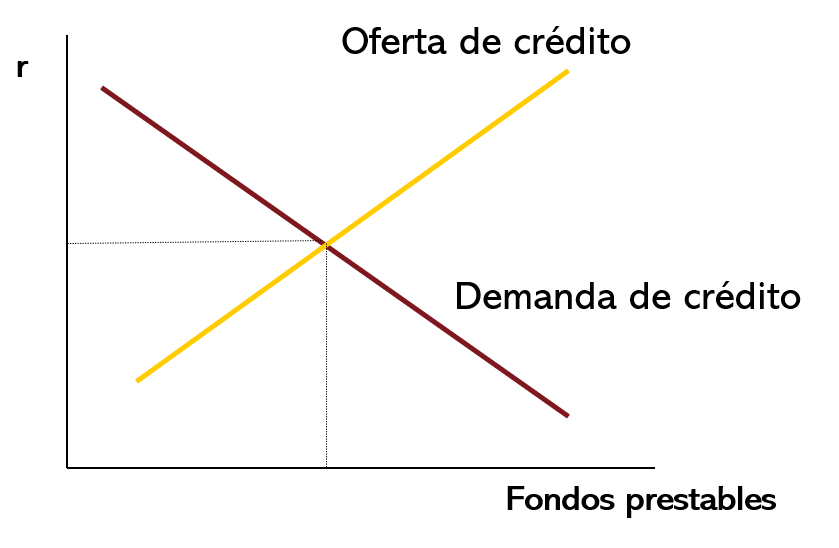
\includegraphics[width=6.5cm]{P46.png}\
%    \begin{itemize}
%        \item La oferta la define el deseo de la gente de ahorrar
%        \item La oferta de fondos depende de la tasa de interés
%        \item La demanda viene dada por la inversión o la demanda de deuda de parte del gobierno
%        \item Ambas decrecen con la tasa de interés
%    \end{itemize}
%\end{frame}


\begin{frame}{ Las funciones del dinero}
    \begin{itemize}
       \item \textbf{Medio de cambio}: el dinero es utilizado como un mecanismo para realizar transacciones. 
  \vspace{1mm}
    \item \textbf{Unidad de cuenta}: el dinero es también una medida que sirve para definir precios así como para registrar activos y deudas.
  \vspace{1mm}  
    \item \textbf{Depósito de valor}: el dinero permite transferir poder adquisitivo del presente al futuro. 
   \end{itemize}
\end{frame}

\begin{frame}
\frametitle{Tipos de dinero}
\begin{itemize}
    \item Durante la mayor parte de la historia de la humanidad se utilizó dinero mercancía (commodity money)
        \begin{itemize}
        \item Mercancías con valor intrínseco que se usaban para comerciar \\
        - Oro, plata, cigarrillos, etc.
        \end{itemize} \vspace{1mm}
    \item Hoy en día, casi todo el dinero es fiduciario (fiat money)               \begin{itemize}
        \item Sin valor intrínseco, pero que se utiliza porque el gobierno lo hace de curso legal (legal tender) \\
        - Pesos, euros, dólares, bonos provinciales (?!), etc.
        \item Ahora es casi natural, pero tomó mucho tiempo \\
        - Problemas de confianza, falsificación, funcionamiento, etc.
        \end{itemize}
\end{itemize}
\end{frame}

\begin{frame}{Commodity money }
            \begin{figure} [H]   
  \centering
  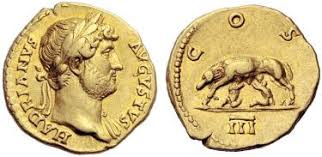
\includegraphics[width=.8\textwidth]{Figures/C32.1.jpg}
      \caption{Monedas carcomidas}
  \label{fig:C32.1}
\end{figure}
\end{frame}

\begin{frame}{Dinero Papel}
    \begin{itemize}
        \item Comienza a usarse en China en el Siglo VII
        \item Antes de los bancos centrales los emitían los bancos 
        
\begin{figure} [H]   
  \centering
  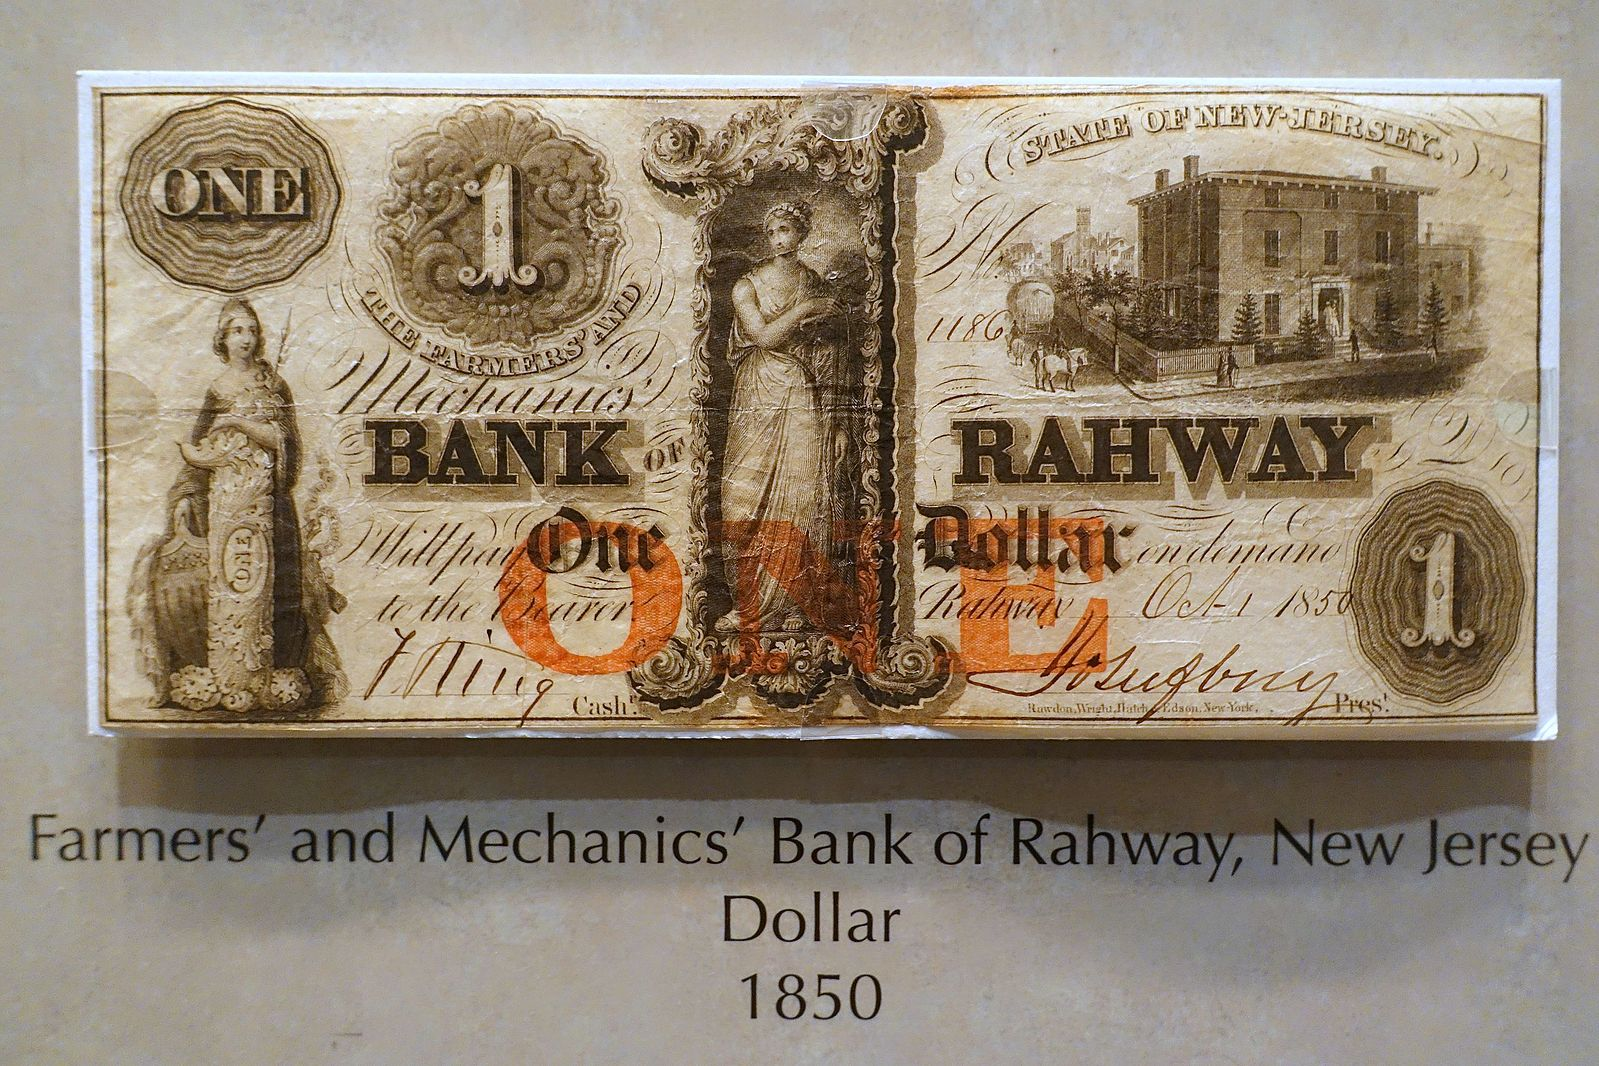
\includegraphics[width=.35\textwidth]{images/C32.2.jpg}
      \caption{Dollar de Bank of Rahway, New Jersey, 1850. Via Wikimedia Commons}
  \label{fig:C32.2}
\end{figure}

\begin{figure} [H]   
  \centering
  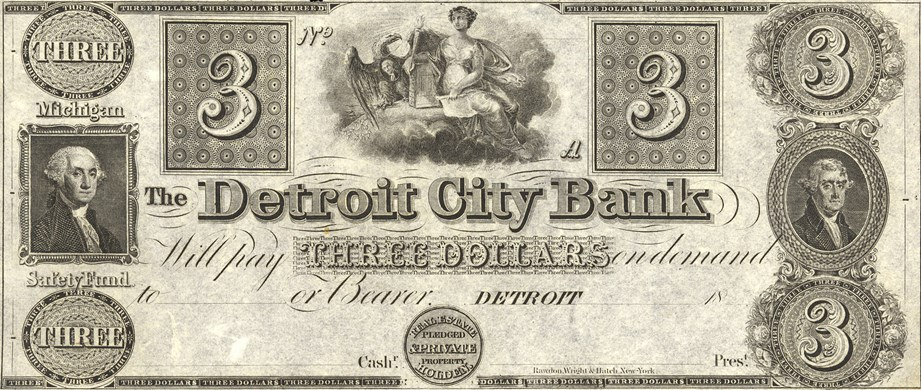
\includegraphics[width=.35\textwidth]{Figures/C32.3.jpeg}
      \caption{Detroit City Bank \$3 Note}
  \label{fig:C32.3}
\end{figure}
\end{itemize}
\end{frame}
        
\begin{frame}{El dinero}
        \begin{figure} [H]   
  \centering
  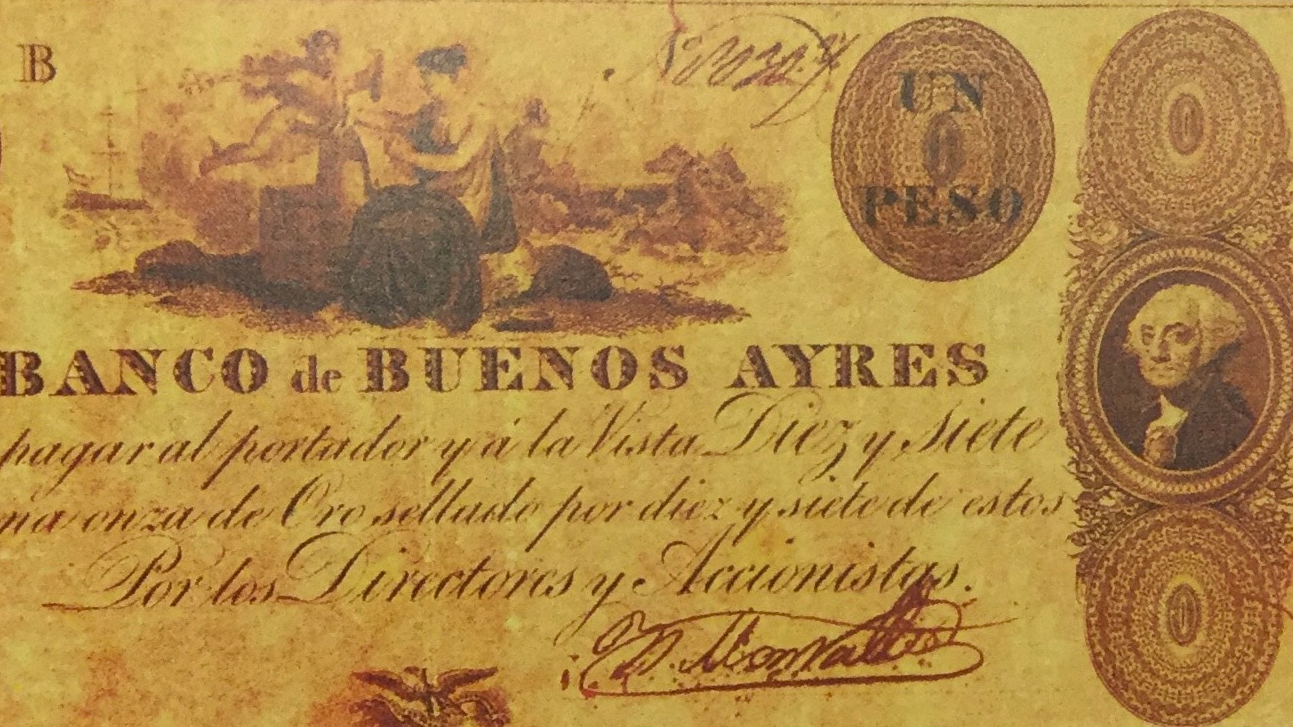
\includegraphics[width=.35\textwidth]{Figures/C32.4.jpg}
      \caption{Billetes emitidos por el Banco Provincia de Buenos Aires}
  \label{fig:C32.4}
\end{figure}

\begin{figure} [H]   
\centering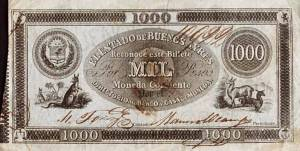
\includegraphics[width=.35\textwidth]{Figures/C32.5.jpg}
\caption{Billetes emitidos por el Banco Provincia de Buenos Aires}
\end{figure}
       \begin{itemize}
           \item  Luego lo monopolizaron los bancos centrales
    \item Y hoy volvemos a la multiplicidad de monedas 
       \end{itemize}     
        \end{frame}
        
\begin{frame}
\frametitle{¿Qué son los bancos?}
\begin{itemize}
    \item Son intermediarios financieros
        \begin{itemize}
        \item Instituciones que reciben fondos de personas y empresas, y los utilizan para comprar bonos o acciones, o para hacer préstamos a otros agentes \\
        - Los bancos piden prestado a los hogares (depósitos), otros bancos, y el banco central \\
        - El interés que pagan por los depósitos (tasa de interés pasiva) es menor que el que cobran en préstamos (tasa de interés activa, lending rate), y así obtienen beneficios
        \end{itemize}
    \item Un tipo particular de intermediario financiero
    ¡sus pasivos son dinero!
\end{itemize}
\end{frame}

\begin{frame}
\frametitle{¿Qué es el Banco Central?}
\begin{itemize}
    \item Un banco particular
        \begin{itemize}
            \item Es generalmente propiedad del gobierno
            \item Actúa como banquero de los bancos comerciales \\
            - Que tienen `reservas' en el Banco Central
            \item Es el único que puede crear moneda de curso legal
        \end{itemize}
    \item Dinero en el sentido amplio
        \begin{itemize}
            \item Base monetaria (base money) o M0 \\
            - Billetes y monedas, más cuentas depositadas en el Banco Central
            \item Depósitos (bank money) \\
            - Dinero creado por los bancos comerciales al extender crédito
        \end{itemize}
\end{itemize}
\end{frame}

\begin{frame}{¿Qué más hace el Banco Central?}
    \begin{itemize}
    \item Crea y regula la cantidad de dinero en la economía
    \vspace{1mm}
    \item Regula la actividad bancaria
    \vspace{1mm}
    \item Es prestamista de última instancia
    \vspace{1mm}
    \item Maneja la política cambiaria 
\end{itemize}
\end{frame}

\begin{frame}{Riesgos que tienen que manejar los bancos}
\begin{itemize}
    \item \textbf{Riesgo de madurez}: como el banco invierte en activos de largo plazo, si la tasa de interés sube, en general el valor de los activos de largo plazo va a caer más que los de corto plazo \vspace{1mm}
    \item \textbf{Riesgo de liquidez}: Es el riesgo de que el activo no se pueda transformar en efectivo (liquidar) sin generar una pérdida financiera \vspace{1mm}
    \item \textbf{Riesgo de default}: Es el riesgo de que los créditos del banco no sean repagados
\end{itemize}
    \end{frame}


\begin{frame}{Apalancamiento (leverage)}
    \begin{itemize}
    \item Un banco es solvente cuando el valor de sus activos supera al de los pasivos
     \item ¿Cómo evaluamos el riesgo de una caida en el valor de los activos?
    \end{itemize}
     \begin{center}
       $ Leverage = \frac{Activo}{\text{Patrimonio Neto}} $
    \end{center} 
    \begin{itemize}
    \item Un coeficiente muy alto, es decir, mucho apalancamiento, implica que gran parte de los activos son financiados con deuda y poco con patrimonio neto. Es decir que los activos se financian con dinero de terceros, no con capital propio.
    \end{itemize}
\end{frame}

\begin{frame}{Ejemplo I}
    \begin{table}[H]
    \centering
%    \vspace{.3cm}
    %\scalebox{.8}{
    \begin{tabular}{|c|c|c|c|}
    \hline
\textbf{Banco}    & \textbf{Activo} & \textbf{Pasivo} & \textbf{Patrimonio Neto}\\
         \hline \hline
         Banco 1 &  100 &  80 & 20\\[1mm]
        \hline
       Banco 2 & 100  &  95& 5\\[1mm]
        \hline
    \end{tabular}
    %}
    \caption{Escenario Inicial}
    \label{inicial}
\end{table}
\end{frame}

\begin{frame}{Ejemplo II}
   \begin{table}[H]
    \centering

%    \vspace{.3cm}
    %\scalebox{.8}{
    \begin{tabular}{|c|c|c|c|}
    \hline
\textbf{Banco}    & \textbf{Activo} & \textbf{Pasivo} & \textbf{Patrimonio Neto}\\
         \hline \hline
         Banco 1 &  90 &  80 & 10\\[1mm]
        \hline
       Banco 2 & 90  &  95& -5\\[1mm]
        \hline
    \end{tabular}
    %}
    \caption{Caída del 10\% del valor de los activos}
    \label{caida10pp}
\end{table} 
\end{frame} 

\begin{frame}{¿Por qué uno quiere leverage?}
\begin{table}[H]
    \centering
%    \vspace{.3cm}
    %\scalebox{.8}{
    \begin{tabular}{|c|c|c|c|}
    \hline
\textbf{Banco}    & \textbf{Activo} & \textbf{Pasivo} & \textbf{Patrimonio Neto}\\
         \hline \hline
         Banco 1 &  110 &  80 & 30\\[1mm]
        \hline
       Banco 2 & 110  &  95& 15\\[1mm]
        \hline
    \end{tabular}
    %}
    \caption{Aumento del 10\% del valor de los activos}
    \label{caida10pp}
\end{table}
\end{frame}

\begin{frame}{Mercado monetario: oferta de dinero \\ La hoja de balance del Banco Central }
\centering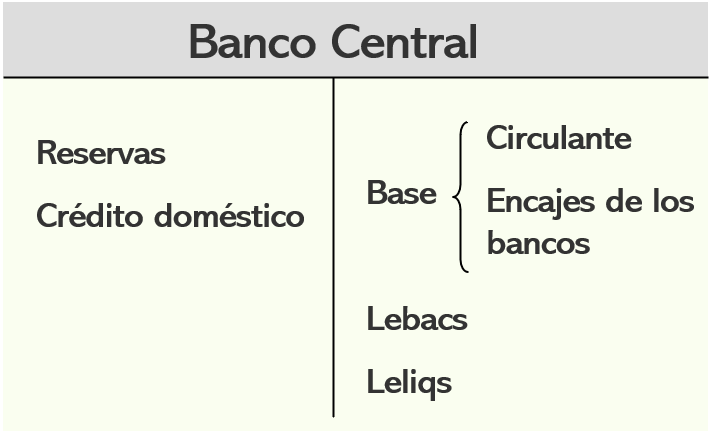
\includegraphics[width=6.5cm]{Figures/P48.png}\
\end{frame}


\begin{frame}{El multiplicador monetario}
    \begin{itemize}
        \item Ejemplo de creación de dinero bancario:  circulante = 100  y  encajes = 10\%
    \end{itemize}

    \vspace{2mm}
    
    \centering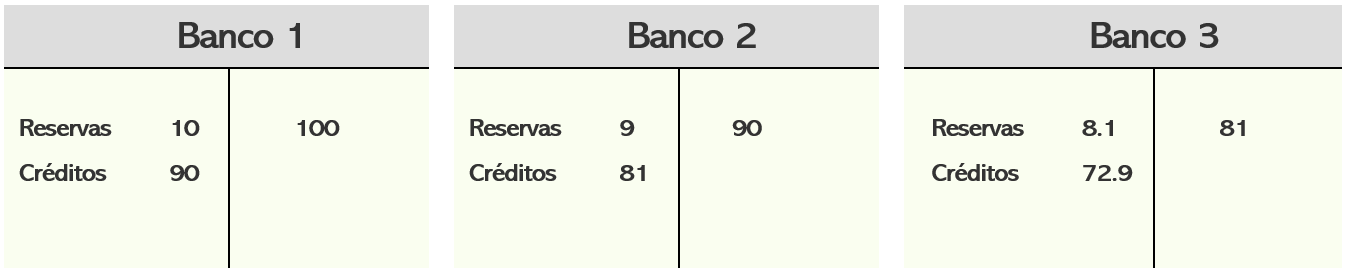
\includegraphics[width=10cm]{Figures/P50.png}\
    
    \vspace{2mm}
    
    \begin{tcolorbox}[width=4in, interior hidden, boxsep=0pt,
                  left=0pt, halign=center, valign=center, right=0pt,
                  bottom=3pt, top=3pt, ]%%
                 \footnotesize{M1 = circulante + depósitos = 100 + 90 + 81 + 72.9 + ..... = 1000}
    \end{tcolorbox}
    \vspace{2mm}
\end{frame}

\begin{frame}{El multiplicador monetario}
    \begin{itemize}
        \item Ejemplo de creación de dinero bancario:  circulante = 100  y  encajes = 20\%
    \end{itemize}
        \vspace{2mm}
    \centering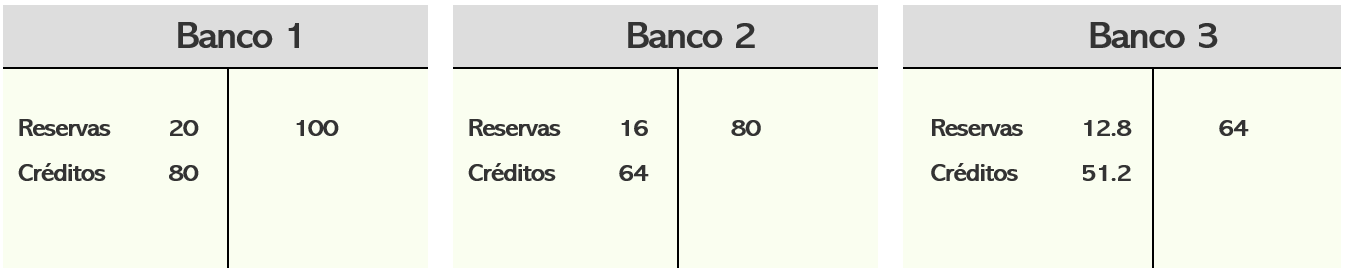
\includegraphics[width=10cm]{Figures/P51.png}\
    \vspace{2mm}
    \begin{tcolorbox}[width=4in, interior hidden, boxsep=0pt,
                  left=0pt, halign=center, valign=center, right=0pt,
                  bottom=3pt, top=3pt, ]%%
                 \footnotesize{M1 = circulante + depósitos = 100 + 80 + 64 + 51.2 + ..... = 500}
    \end{tcolorbox}
        \vspace{2mm}
    \begin{itemize}
        \item Los encajes se usan para regular la cantidad de dinero
        \item ¡Subimos los encajes y cae la cantidad de dinero!  \Large\Cooley[][yellow!60!white]
        \end{itemize}
\end{frame}


\begin{frame}{Los agregados monetarios M}
     \begin{itemize}
        \item M0 = Base monetaria = Circulante + Encajes bancarios
        \item M1 = Circulante + Depósitos en cuenta corriente
        \item M2 = M1 + Caja de Ahorro
        \item M3 = M2 + Plazo Fijo
        \item M? = M3 + saldos de tarjetas?, programa de millajes? 
        \item etc.
    \end{itemize}
\end{frame}

\begin{frame}{Mercado monetario: la demanda de dinero}
    \begin{itemize}
        \item La demanda de dinero es lo que la gente demanda de dinero, es cuánto dinero desea tener la sociedad
        \item Se explica por dos motivos principalmente: por motivo transacción y por motivo especulación
        \begin{itemize}
        \item Por transacciones $\Rightarrow P*Y \Rightarrow$ a mayores precios o mayor nivel de actividad aumenta la demanda de dinero por transacciones
        \item Costo de oportunidad $\Rightarrow i \Rightarrow $ la demanda de dinero depende negativamente de la tasa de interés que es el costo de oportunidad del dinero
    \end{itemize}
    \end{itemize}
\end{frame}


\begin{frame}{La teoría cuantitativa del dinero}
\begin{itemize}
        \item La teoría cuantitativa del dinero
        \vspace{0.3cm}
                \begin{tcolorbox}[width=4in,
                  interior hidden,
                  boxsep=0pt,
                  left=0pt,
                  right=0pt,
                  top=2pt,
                  ]%%
                                 $$M*V(i)=P*Y$$
                \end{tcolorbox} 
        \item Si el producto está dado por el mercado de trabajo y la tasa de interés por el mercado de crédito
        \item La ecuación se transforma en una ecuación de determinación de los precios
    \end{itemize}
    \begin{itemize}
    \begin{tcolorbox}[width=4in,
                  interior hidden,
                  boxsep=0pt,
                  left=0pt,
                  right=0pt,
                  top=2pt,
                  ]%%
                                 $$P=\left(\frac{M^{*} V}{Y}\right)$$
                \end{tcolorbox} 
    \end{itemize}
    \begin{itemize}
        \item Aumentos en \textit{M} son seguidos por aumentos en \textit{P}
    \end{itemize}
\end{frame}

\begin{frame}{Inflación}
    \begin{itemize}
    \item La TCD con tasas de crecimiento: \\
$$\frac{\vartriangle M}{M} + \frac{\vartriangle V}{V} = \frac{\vartriangle P}{P} + \frac{\vartriangle Y}{Y}$$ \vspace{1mm}
    \item Sabiendo que la inflación es $\pi = \frac{\vartriangle P}{P}$, luego la inflación es: \\
    $$\pi = \frac{\vartriangle M}{M} - \frac{\vartriangle Y}{Y} + \frac{\vartriangle V}{V}$$ \vspace{1mm}
    \item La tasa de crecimiento del dinero es un predictor esencial de la inflación
    %\item Y consecuentemente también lo son los déficit fiscales u otro motivo de expansión monetaria
    \end{itemize}
\end{frame}

\begin{frame}{Evolución de la base monetaria vs. IPC}
\centering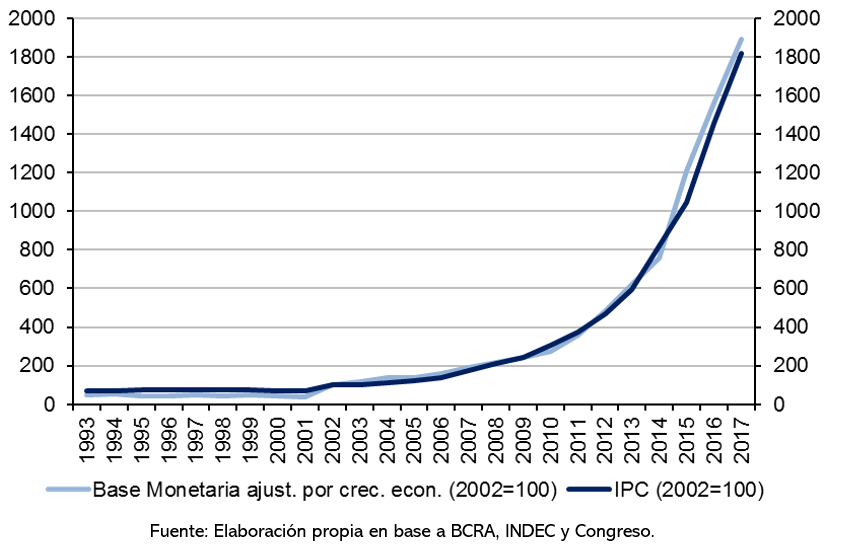
\includegraphics[width=11cm]{Figures/P55.png}\
\end{frame}

\begin{frame}{El equilibrio del mercado monetario}
\centering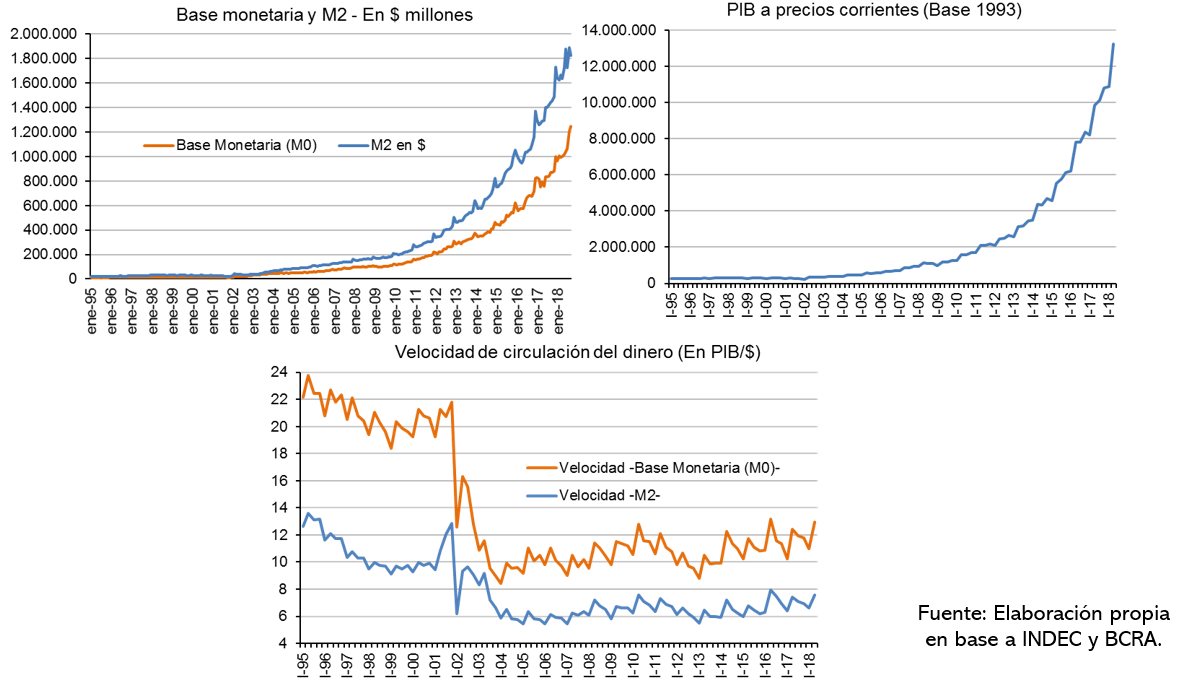
\includegraphics[width=11cm]{Figures/P56.png}\
\end{frame}

\begin{frame}{El equilibrio del mercado monetario II}
\centering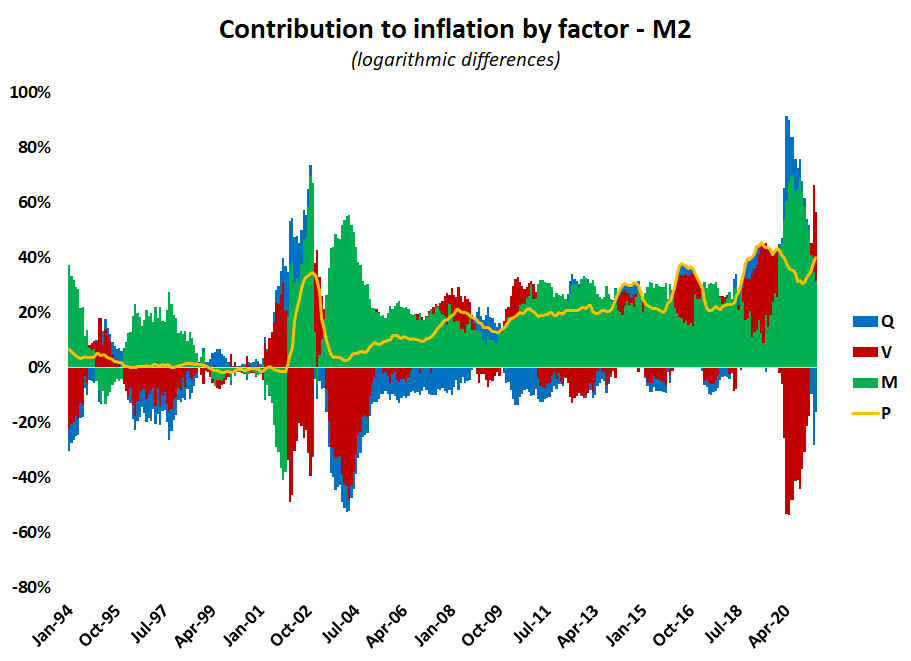
\includegraphics[width=10cm]{Figures/inflation contribution by factor.png}\
\end{frame}

\begin{frame}{Malas teorías de la inflación}
    \begin{itemize}
        \item Realmente solo en Argentina se repiten estas ideas
            \begin{itemize}
        \item Es la puja distributiva
        \item Es culpa del dolar
        \item El aumento de las tarifas como generadoras de inflación
        \item Los supermercados aumentan los márgenes de ganancia y eso explica por qué aumentan los precios
            \end{itemize}
        \item Ninguna de estas teorías puede explicar la inflación
        \item Obviamente se mueven con la inflación y por eso es fácil confundirse, recuerden el problema de la variable omitida
        \item Y todo esto puede afectar las expectativas que se forman las personas acerca de los precios y, se complica más la cosa
        \item Por ejemplo: si las expectativas no se alinean, la política monetaria va a tener que ser más dura para bajar la inflación
    \end{itemize}
\end{frame}

\begin{frame}{ La relación entre política monetaria y precios...}
\centering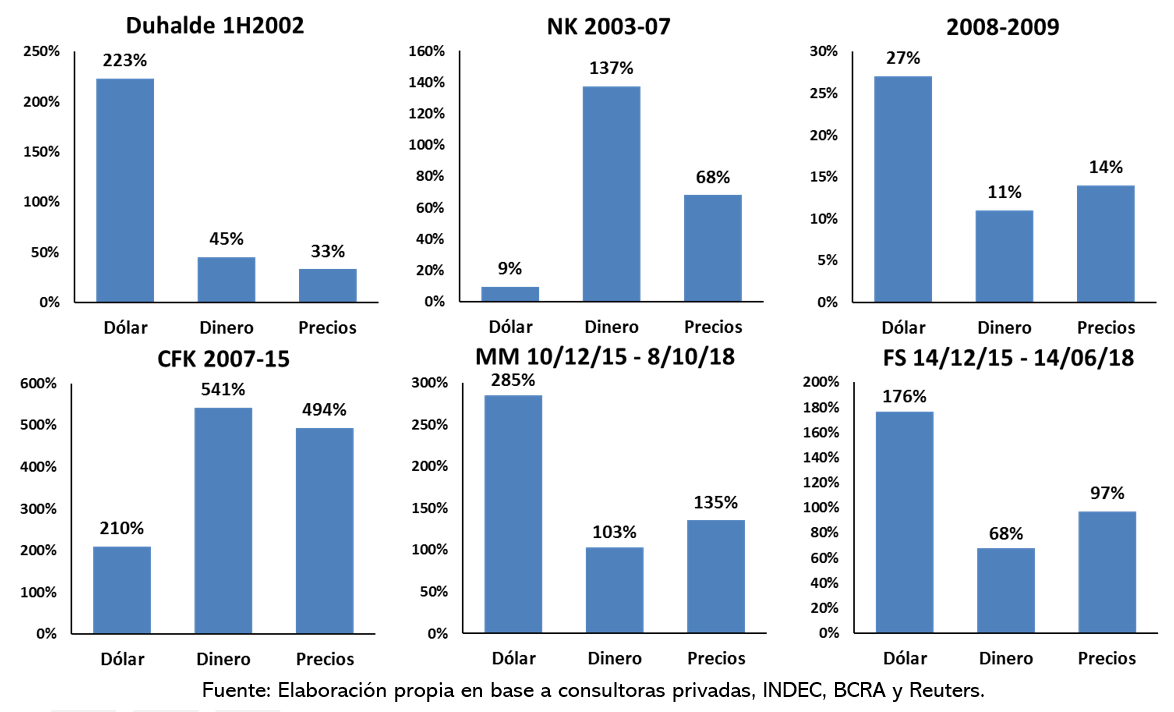
\includegraphics[width=11cm]{Figures/P57.png}\
\end{frame}

\begin{frame}{Consensos sobre la Política Monetaria}
\begin{itemize}
    \item Mishkin (2007) comenta que hay 6 consensos 
    \begin{itemize}
        \item No hay relación de largo plazo entre la política monetaria y el producto
        \item Expectativas son importantes para la efectividad de la política monetaria
        \item La inflación es mala
        \item La política monetaria tiene un problema de inconsistencia temporal
        \item La independencia del Banco Central mejora la efectividad de la política monetaria
        \item Un ancla nominal fuerte es clave para generar una buena política monetaria
    \end{itemize}
\end{itemize}
\end{frame}

\begin{frame}{¿Cómo controlan los Bancos Centrales las expectativas?}
    \begin{itemize}
 \item Pero igual los bancos centrales quieren controlar las expectativas
 \item Hay tres maneras de hacerlo
  \begin{itemize}
    \item Fijando la cantidad de dinero
    \item Fijando el tipo de cambio
    \item Fijando la tasa de interés y apuntando a un valor de inflación
   \end{itemize}
  \end{itemize}
 
  \centering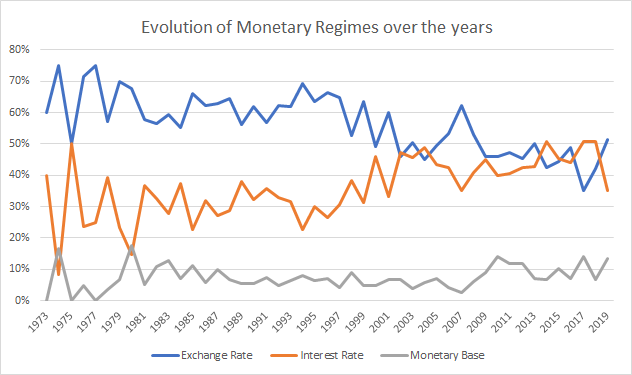
\includegraphics[width=7cm]{image (5).png}\
  
\end{frame}

\begin{frame}{La inflación en el mundo}
    \centering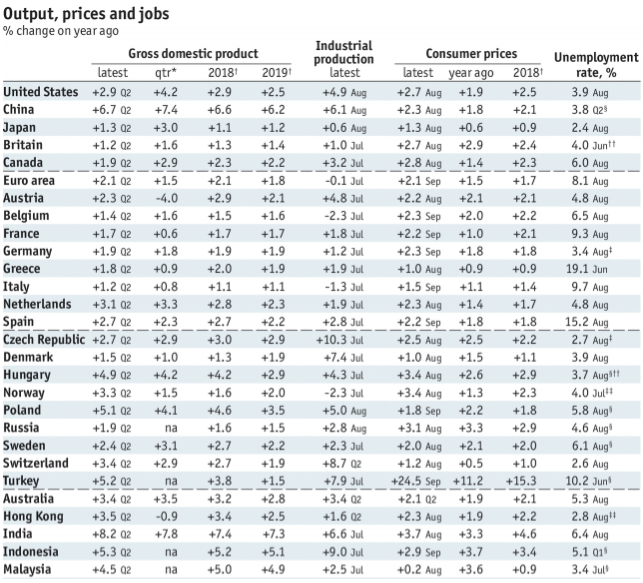
\includegraphics[width=8cm]{P70.png}\
\end{frame}


\begin{frame}{Continuación}
    \centering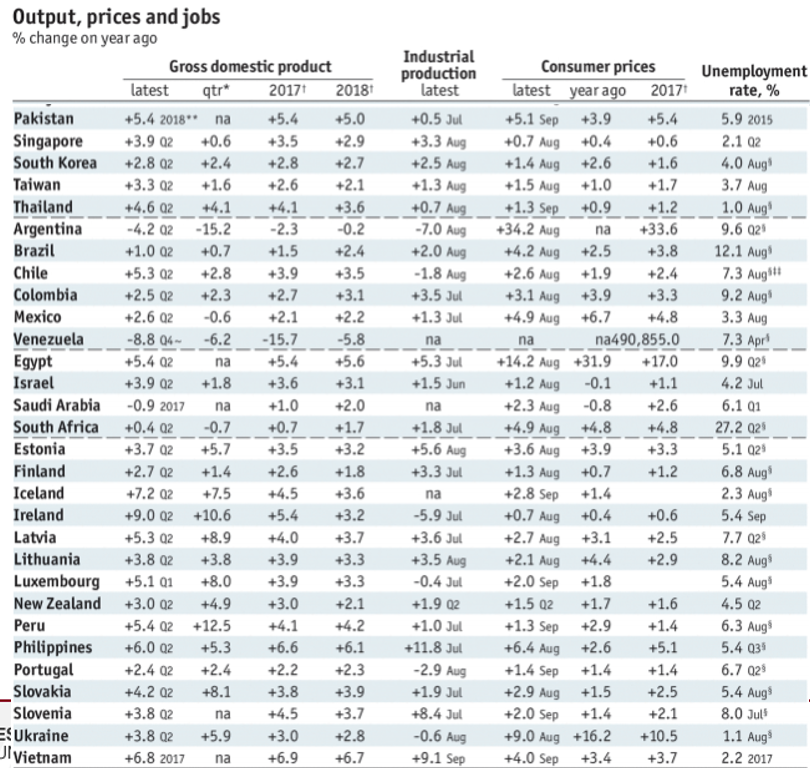
\includegraphics[width=8cm]{P71.png}\
\end{frame}

\begin{frame}{La inflación en Argentina en una perspectiva histórica}
\centering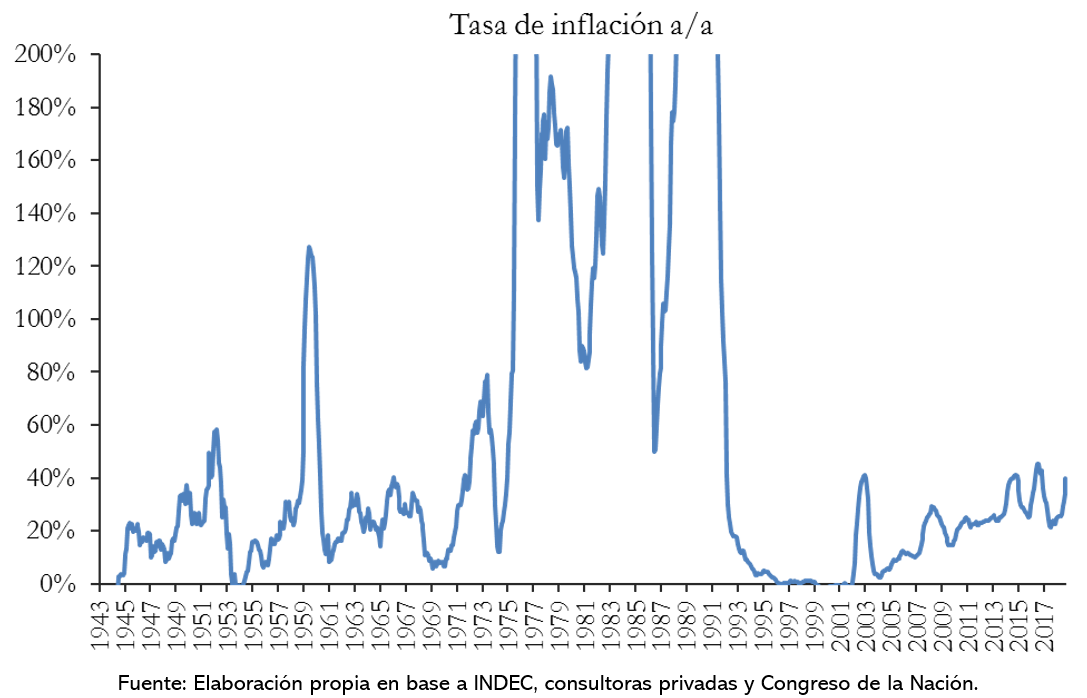
\includegraphics[width=10cm]{Figures/P59.png}\
\end{frame}

\begin{frame}{¿Qué nos pasa?}
\centering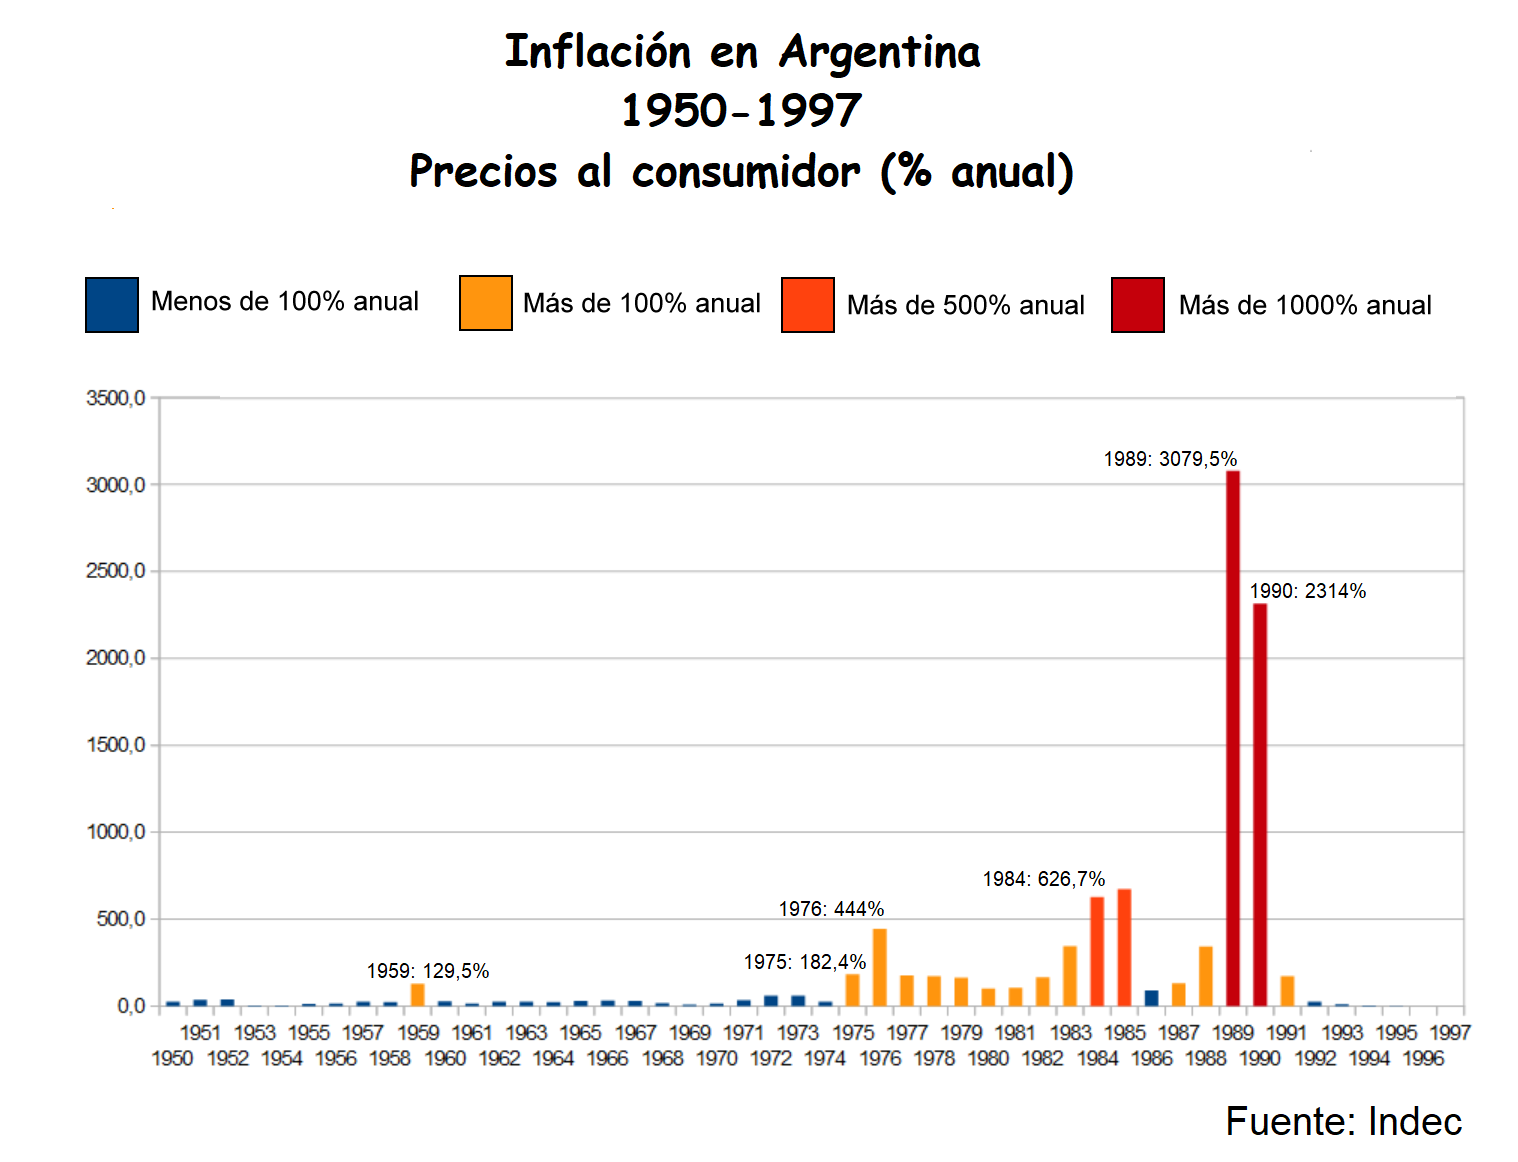
\includegraphics[width=10cm]{Figures/infarg.png}\
\end{frame}

\begin{frame}{ Argentina: crecimiento de M }
\centering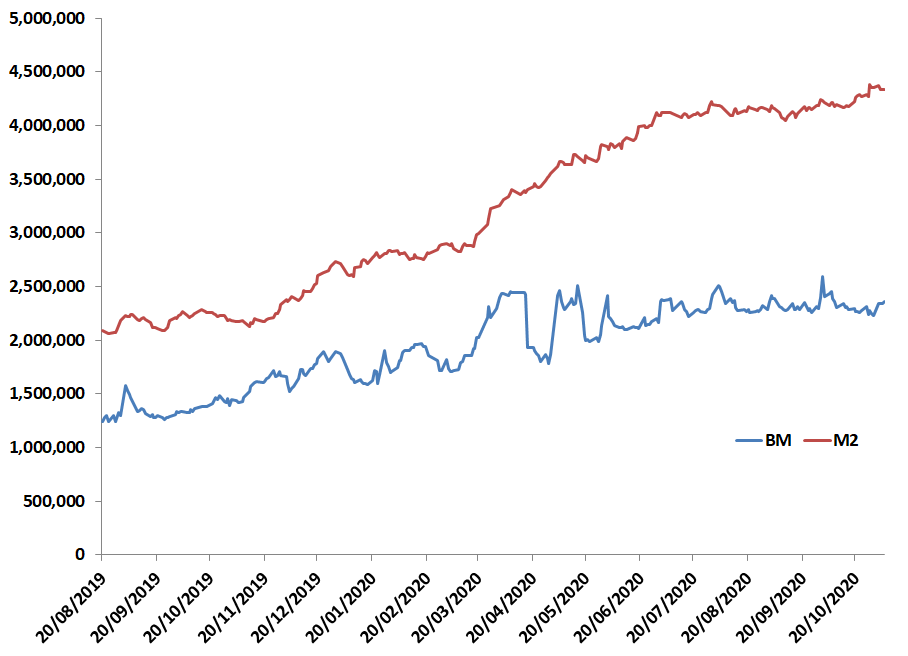
\includegraphics[width=10cm]{Figures/agregados.png}
\end{frame}

\begin{frame}{Inflación y distribución del ingreso}
    \begin{figure} [H]   
\centering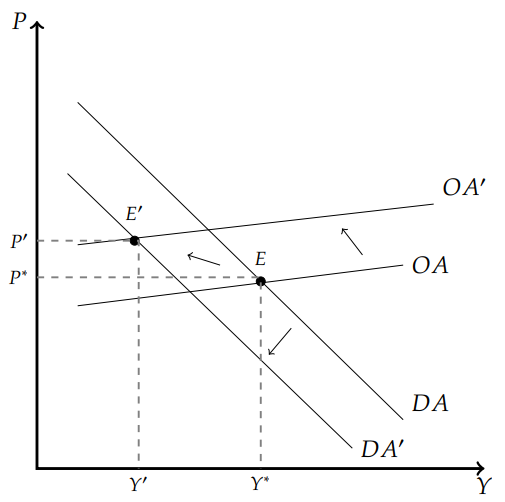
\includegraphics[width=0.9\textwidth]{Figures/C33.10.png}\
\caption{\textbf{Efectos redistributivos}}
\end{figure}
\end{frame}

%\begin{frame}{Después de 2008 muchos bancos centrales emitieron también mucho}
%\centering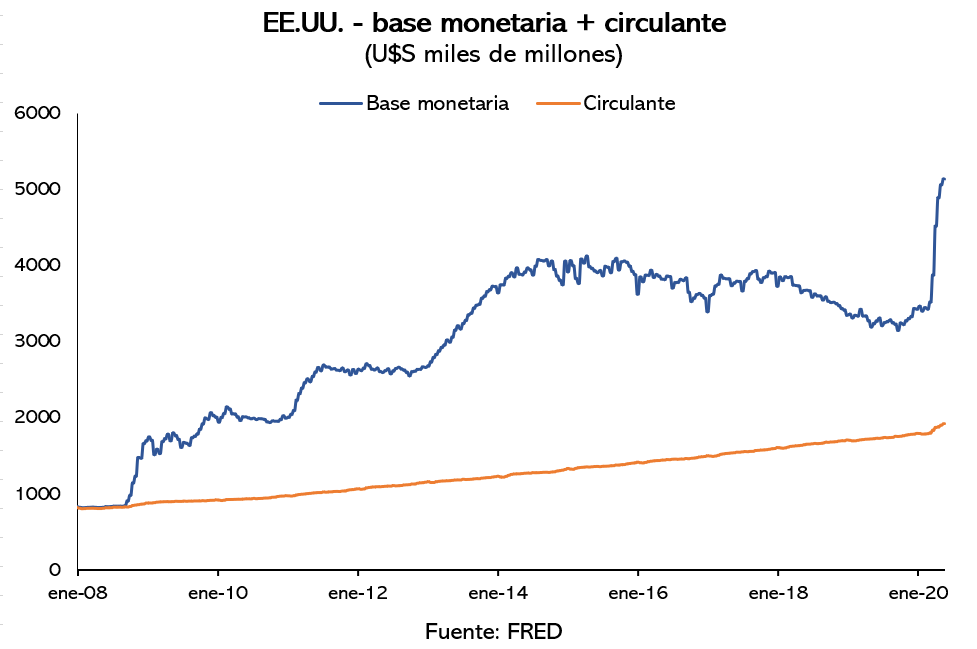
\includegraphics[width=8cm]{P62b.png}\
%\begin{itemize}
%   \item Diferente emitir que comprar activos    
%   \item Quantitative easing inyecto liquidez pero no "mas medios de pagos netos"
%    \item Lo mismo se aplica a compras de reservas contra Lebacs
%\end{itemize}
%\end{frame}

\begin{frame}
\frametitle{¿Por qué emitir dinero!?}
\begin{itemize}
    \item La inflación puede funcionar como variable de ajuste \vspace{2mm}
    \item El gobierno se queda con el impuesto inflacionario
    \begin{itemize}
        \item Al emitir dinero, el gobierno hace que el salario de la gente valga menos
    \end{itemize}
\end{itemize}
\end{frame}

\begin{frame}
\frametitle{¿Cómo funciona el impuesto inflacionario?}
\begin{itemize}
    \item El gobierno le debe pagar a Gaby y a Maxi \$100 a cada uno. 
    \item Por otro lado, en la economía hay 20 flynn paffs. Precio de un flynn paff: \$5.
    \item Solo tiene \$100 y se los da a Gaby. ¿Y a Maxi? ¡A imprimir!
    \item Ahora hay \$200 dando vueltas, pero los mismos 20 flynn paffs. Precio de un flynn paff: \$10
    \item Conclusión: ¡Cada uno puede comprar 10!
\end{itemize}
\end{frame}

%\begin{frame}
%\frametitle{18. ¿Cómo funciona el impuesto inflacionario?}
%\begin{itemize}
%    \item El gobierno le debe pagar a Gaby y a Maxi \$100 a cada uno. 
%    \item Por otro lado, en la economía hay 20 flynn paffs. Precio de una flynn paff: \$5.
%    \item Solo tiene \$100 y se los da a Gaby. ¿Y a Maxi? ¡A imprimir!
%    \item Ahora hay \$200 dando vueltas, pero las mismas 20 flynn paffs. Precio de un flynn paff: \$10
%    \item Conclusión: ¡Cada uno puede comprar 10!
%\end{itemize}
%\end{frame}

\begin{frame}
\frametitle{Emisión y señoreaje}
\begin{itemize}
    \item Recordemos que los gobiernos pueden financiarse imprimiendo dinero
        \begin{itemize}
        \item Bonos que el Banco Central se ve obligado a aceptar \\
        - Monetización de la deuda
        \end{itemize}
    \vspace{2mm}
    \item Uso del señoreaje
\begin{itemize}
        \item Retorno por la creación de dinero
        \item Como la expansión monetaria típicamente conlleva a una subida de precios, funciona como un impuesto inflacionario sobre tenedores de dinero 
        \end{itemize}
\end{itemize}
\end{frame}

\begin{frame}{Cambios en la demanda y oferta de dinero}
    \begin{itemize}
            \item Un aumento en la demanda de dinero sube las tasas
            \item Un aumento en la oferta de dinero baja las tasas
            \item Es decir que, potencialmente, se moverá la demanda agregada 
        \end{itemize}
    \vspace{0.3cm}
    \centering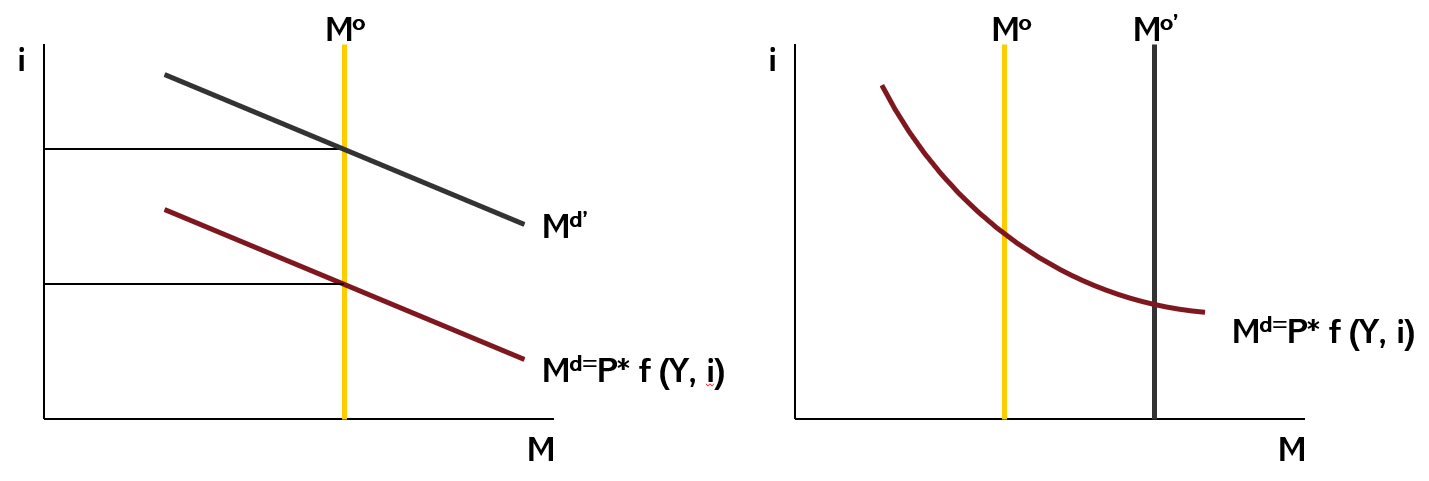
\includegraphics[width=11cm]{Figures/P62.png}\
\end{frame}

\begin{frame}{Funcionamiento del mercado monetario}
    \begin{itemize}
    \item La mayoría de los bancos centrales fijan la tasa, pero es lo mismo:
    \end{itemize}
    \vspace{0.4cm}
    \centering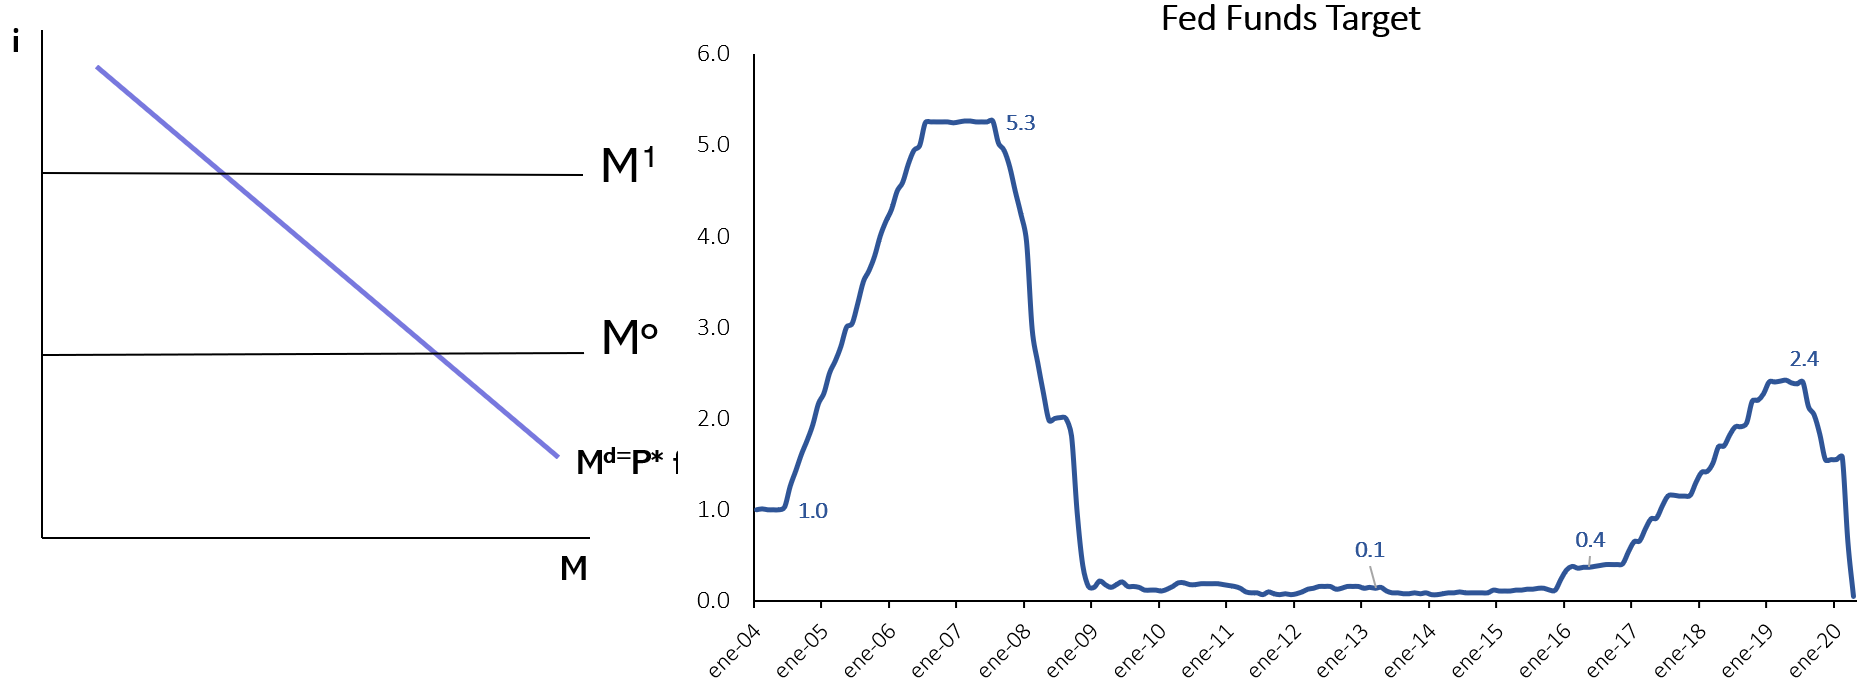
\includegraphics[width=11cm]{Figures/P63.png}\\
\end{frame}

\begin{frame}
\frametitle{Tasas de interés}
\begin{itemize}
    \item Tasa de interés nominal $i_t$
    \begin{itemize}
        \item ¿Cómo cambia, en términos de una moneda en particular, el valor de lo que presto o pido prestado? \\
        - Un préstamo de \$V este año genera unos rendimientos de \\ \$(1 + $i_t$)V el próximo año
    \end{itemize} \vspace{4mm}
    \item Tasa de interés real $r_t$
    \begin{itemize}
        \item ¿Qué pasa si hay inflación?
        \item Tasas de interés expresadas en términos de una canasta de bienes \\
        - Tasa que le importa a las personas sin ilusión monetaria
        \end{itemize}
    \end{itemize}
\end{frame}

%\begin{frame}
%\frametitle{22. De nominal a real}
%¿Cómo pasamos de uno (que observamos) al otro (que no lo observamos)?
%\begin{center}
%\includegraphics[scale=0.55]{Magistrales/Tema_13.3_denominalareal.jpg}
%\end{center}
%\end{frame}

\begin{frame}
\frametitle{Pensando en la relación}
\begin{itemize}
    \item Entonces tenemos que:\\
    \vspace{2mm}
    \begin{center}
        $1+r_t=(1+i_t)\frac{P_t}{P_{t+1}^{e}}$
    \end{center}
        \vspace{2mm}
    \item Recordemos \\      
    \begin{center}
        $\pi_t=\frac{P_t - P_{t-1}}{P_{t-1}}=\frac{P_t}{P_{t+1}} - 1 $ \\
    \vspace{2mm}
            $\frac{P_t}{P_{t-1}}= \pi_t + 1 $
    \end{center}
\begin{itemize}
    \item Si $\frac{P_t}{P_{t-1}}$ es igual a $(\pi_t + 1)$, podemos establecer:
    \vspace{2mm}
        \begin{center}
            $\frac{P_{t+1}^e}{P_{t}}= \pi_{t+1}^e + 1 $
    \end{center}
\end{itemize} 
\end{itemize}
\end{frame}

\begin{frame}
\frametitle{Intereses e inflación}
\begin{itemize}
    \item Podemos simplificar la relación entre las tasas de interés y la inflación esperada:
    \vspace{2mm}
    \begin{center}
        $1+r_t=\frac{(1+i_t)}{(1+\pi_{t+1}^e)}$
    \end{center}
        \vspace{2mm}
    \item Suponiendo que el valor de las variables no es demasiado grande... $\frac{(1+x)}{(1+y)} \approx 1 + x - y $\\
    - Sabemos que si x, y son pequeñas:     
    \item ... obtenemos la ecuación de Fisher: 
    \vspace{2mm}
        \begin{center}
        $r_t \approx i_t - \pi_{t+1}^e$
    \end{center}
\end{itemize}
\end{frame}


\begin{frame}
\frametitle{Maxi y Gaby}
\begin{itemize}
    \item Maxi le pidió a Gaby \$100 prometiendo pagar \$110, entonces la tasa nominal de interés es:
    \vspace{2mm}
    \begin{center}
        $i_{HOY}=\frac{\$110 - \$100}{\$100} * 100 = 10\%$
    \end{center}
        \vspace{2mm}
    \item Si la tasa de inflación esperada para mañana es 5\%, entonces la tasa de interés real es: \\
    \begin{center}
        $r_{HOY} = i_{HOY}-\pi_{MAÑANA}^e$ \\
        \vspace{2mm}
        $r_{HOY} = 10\%-5\% $ \\
        \vspace{2mm}
        $r_{HOY} = 5\%$
    \end{center}
\end{itemize}
\end{frame}


%\begin{frame}{}
%    \centering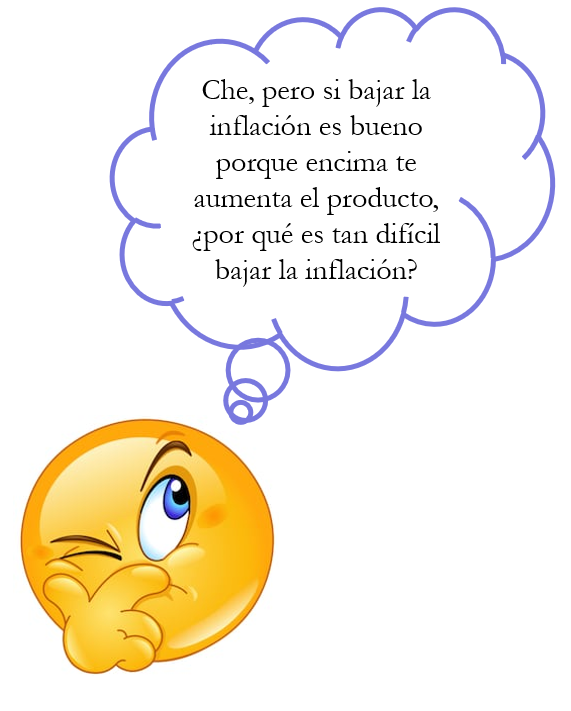
\includegraphics[width=6cm]{PEmoticon.png}\
%\end{frame}


%\begin{frame}{La Presidencia de Macri en dos tiempos. Tiempo I}
%\centering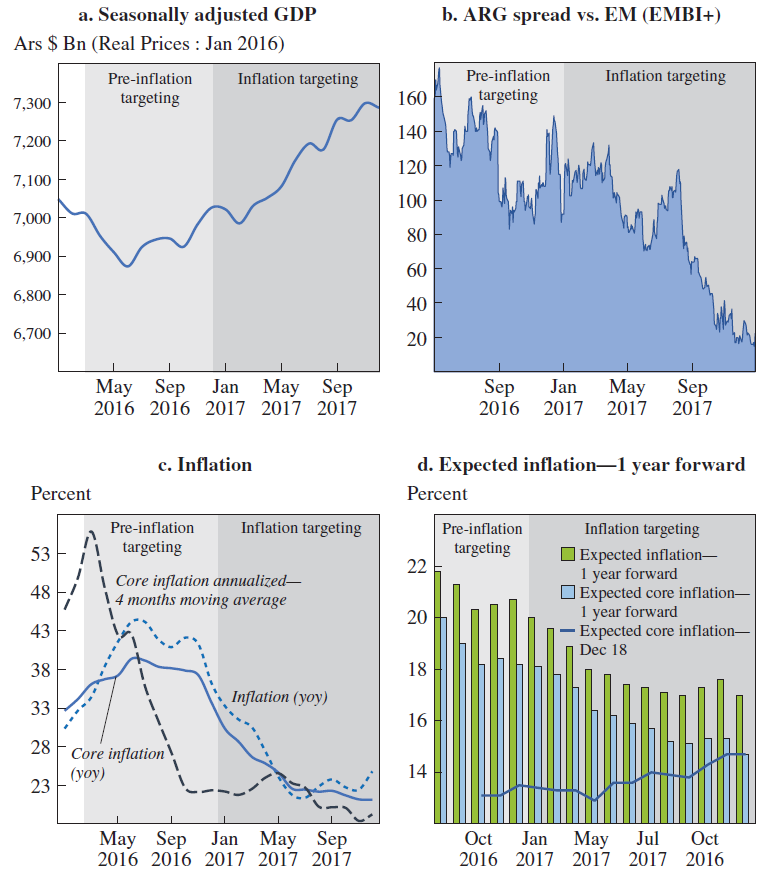
\includegraphics[width=7cm]{MM1.png}\
%\end{frame}

%\begin{frame}{La Presidencia de Macri en dos tiempos. Tiempo II}
%\centering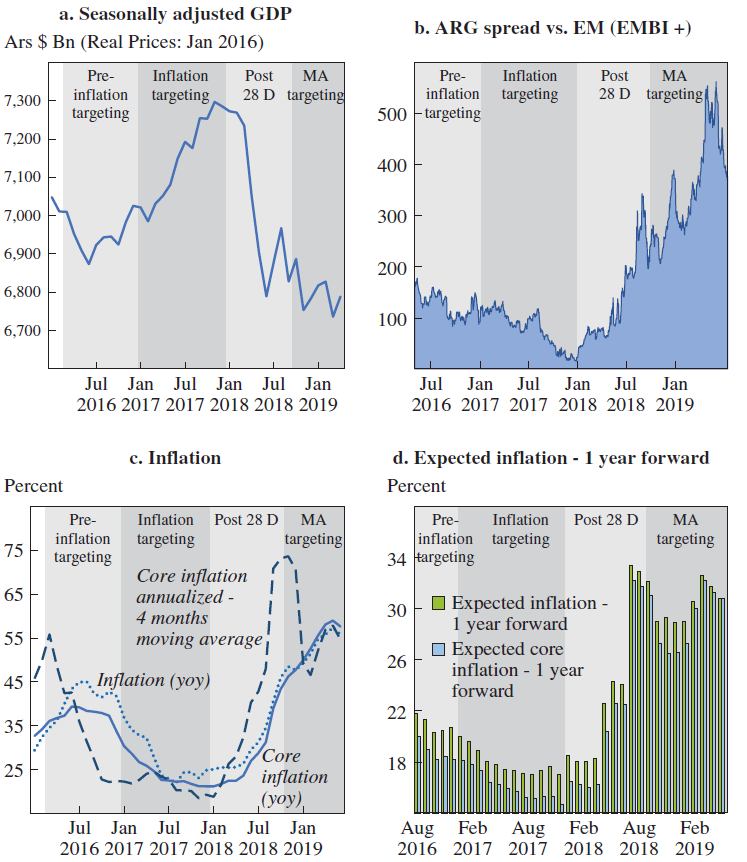
\includegraphics[width=6.5cm]{MM2.png}\
%\end{frame}

%\begin{frame}{Inflación y crecimiento}
%    \begin{figure} [H]   
%\centering\includegraphics[width=1\textwidth]{images/C33.11.png}\
%\caption{\textbf{Efectos sobre el crecimiento de largo plazo}}
%\end{figure}
%\end{frame}

%\begin{frame}{}
%\centering 	\huge \textbf{El mecano } 
%\vspace{2mm}
%\hrule
%\end{frame}
%------------
%---------------------------------------------------------------------------%

\begin{frame}{Ciclos Económicos: un repaso del funcionamiento del mecano}
\centering\includegraphics[width=11cm]{Figures/P18.png}\
\end{frame}

\begin{frame}{Política monetaria en el mundo clásico}

    \begin{itemize}
        \item “Aumenta la demanda agregada” al meter liquidez en el sistema 
       \item Pero el producto está dado por la oferta agregada
        \item Por lo que el aumento en la demanda presiona sobre los precios
        \item Lo que lleva a que los precios aumenten proporcionalmente a lo que aumentó la cantidad de dinero
       \item Oferta y demanda de dinero simplemente se corren para encontrar el equilibrio en el mismo nivel.
        \item $\uparrow M V(i)=\uparrow P Y$ 
       \item Dicotomía clásica (“Neutralidad del dinero”) - $(Y \text { e } i \text { constante, } M \rightarrow P)$
    \end{itemize}
\end{frame}

\begin{frame}{¿Se acuerdan cómo se recauda el impuesto inflacionario?}
    \begin{itemize}
        \item El gobierno emite un dinero
        \item Esto aumenta lo precios
        \item Ese aumento de precios hace que los tenedores de pesos puedan consumir menos
        \item De esa manera, parte del producto lo apropia el Estado
    \end{itemize}
\end{frame}

\begin{frame}{Política monetaria en el mundo keynesiano}
    \begin{itemize}
        \item Ahora “aumenta la demanda agregada” pero ahora esto baja la tasa de interés y lleva a un aumento en el producto.
        \item El dinero excedente reduce la tasa de interés en el mercado de crédito
       \item $\uparrow M V(i) \downarrow=\bar{P} Y \uparrow$
       \item (P constante $, M \rightarrow i, i \rightarrow Y)$
    \end{itemize}
\end{frame}

\begin{frame}{¿Es efectiva la política monetaria?}
    \begin{itemize}
        \item Depende del contexto si los precios se mueven rápido no va a lograr mucho, si los precios son "rígidos" tendrá más impacto. 
        \item En definitiva es una cuestión de contexto.
        \item Podríamos presumir que la política monetaria en Argentina sería menos efectiva que en los EEUU
    \end{itemize}
\end{frame}

\begin{frame}{¿Cómo funcionan la política monetaria y la fiscal?}
    \centering\includegraphics[width=11cm]{P81.png}\
\end{frame}

\begin{frame}{Maneras de pensar la política monetaria}
    \begin{itemize}
        \item La política monetaria se apoya en un “ancla nominal”: tipo de cambio, cantidad de dinero o metas de inflación.
        \item ¿Discreción o reglas?
        \item Mayor discreción lleva a más inflación
        \item Mayor preocupación por el producto lleva a más inflación
            \item Paradoja: cuanto más creíble es un banquero central, más discrecional puede ser
            %\item  Por eso el 28D fue tan trascendental en la presidencia de Macri. 
        \end{itemize}
\end{frame}
\begin{frame}{¡Se viene el mecano en gráficos!}

\begin{itemize}
    \item Vamos a usar lo que vimos hasta ahora para darle una representación gráfica al sistema 
    \item Esto va implicar graficar conjuntamente el mercado de bienes, dinero, crédito y trabajo
    \item En los gráficos que siguen usamos la siguiente terminología, 
    \begin{itemize}
        \item P: el nivel de precios de la economía
        \item Q: el nivel del producto
        \item i: la tasa de interés nominal
        \item M: la cantidad de dinero
        \item FP: la cantidad de crédito
        \item w: el salario nominal
        \item T: el nivel de empleo de la economía
    \end{itemize}
\end{itemize}

\end{frame}


\begin{frame}{El mecano en el mundo clásico}
    
\begin{center}
\begin{figure}[H]
\renewcommand{\figurename}{Figure}
\begin{center}
    \begin{minipage}[b]{0.45\textwidth}
        \begin{center}
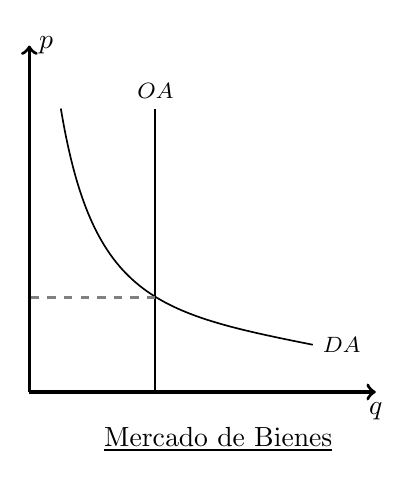
\begin{tikzpicture}[scale=0.4]
\draw[very thick,<-] (0,11)--(0,0);
\draw[very thick,->] (0,0)--(11,0) node[below]{$q$};
\node[right] at (0,11) {$p$};


\node[] at(6,-1.5) {\underline{Mercado de Bienes}};
\draw[semithick] (1,9).. controls (2,3) and (4, 2.5) .. (9, 1.5) node [right]{\footnotesize $DA$};
\draw[semithick](4, 0)--(4, 9) node [above]{\footnotesize $OA$};

\draw[thick, gray, dashed] (4,3)--(0,3);
\end{tikzpicture}
\end{center}
     \end{minipage}
  %  \hfill
    \begin{minipage}[b]{0.45\textwidth}
    \begin{center}
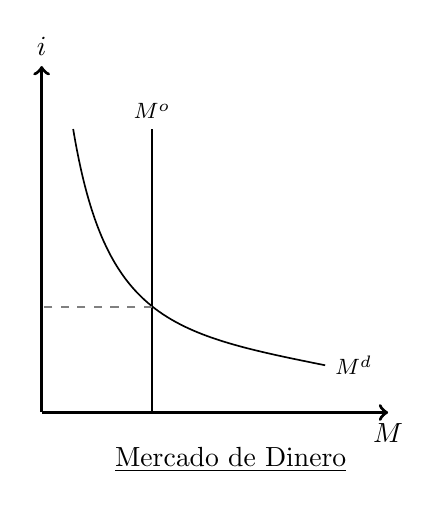
\begin{tikzpicture}[scale=0.4]
\draw[very thick,<-] (0,11) node[above]{$i$}--(0,0);
\draw[very thick,->] (0,0)--(11,0) node[below]{$M$};
\node[right] at (0,11) {};

\node[] at(6,-1.5) {\underline{Mercado de Dinero}};
\draw[semithick] (1,9).. controls (2,3) and (4, 2.5) .. (9, 1.5) node [right]{\footnotesize $M^{d}$};
\draw[semithick](3.5, 0)--(3.5, 9) node [above]{\footnotesize $M^{o}$};

 \draw[thick, gray, dashed] (3.5,3.35)--(0,3.35);

\end{tikzpicture}
\end{center}
    \end{minipage}
\end{center}
\vspace{0.7cm}
\label{fig:C35.3}
\end{figure}
\end{center} 
  
  
\end{frame}



\begin{frame}{El mecano en el mundo keynesiano}
 
 \begin{center}
\begin{figure}[H]
\renewcommand{\figurename}{Figure}
\begin{center}
    \begin{minipage}[b]{0.45\textwidth}
        \begin{center}
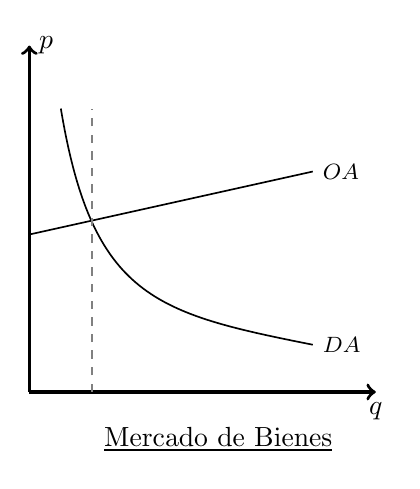
\begin{tikzpicture}[scale=0.4]
\draw[very thick,<-] (0,11)--(0,0);
\draw[very thick,->] (0,0)--(11,0) node[below]{$q$};
\node[right] at (0,11) {$p$};


\node[] at(6,-1.5) {\underline{Mercado de Bienes}};
\draw[semithick] (1,9).. controls (2,3) and (4, 2.5) .. (9, 1.5) node [right]{\footnotesize $DA$};
\draw[semithick](0, 5)--(9,7) node [right]{\footnotesize $OA$};
 \draw[thick, gray, dashed] (2,0)--(2,9);
\end{tikzpicture}
\end{center}
     \end{minipage}
  %  \hfill
    \begin{minipage}[b]{0.45\textwidth}
    \begin{center}
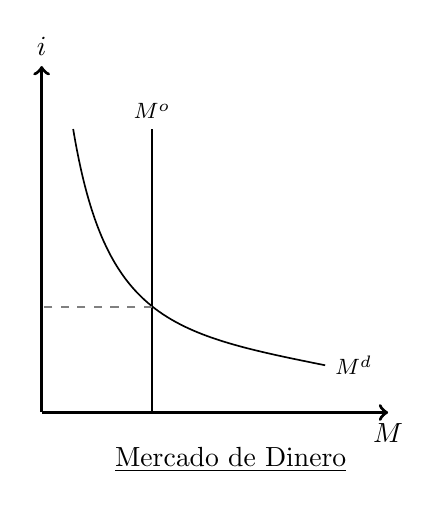
\begin{tikzpicture}[scale=0.4]
\draw[very thick,<-] (0,11) node[above]{$i$}--(0,0);
\draw[very thick,->] (0,0)--(11,0) node[below]{$M$};
\node[right] at (0,11) {};


\node[] at(6,-1.5) {\underline{Mercado de Dinero}};
\draw[semithick] (1,9).. controls (2,3) and (4, 2.5) .. (9, 1.5) node [right]{\footnotesize $M^{d}$};
\draw[semithick](3.5, 0)--(3.5, 9) node [above]{\footnotesize $M^{o}$};

 \draw[thick, gray, dashed] (3.5,3.35)--(0,3.35);

\end{tikzpicture}
\end{center}
    \end{minipage}
\end{center}
\vspace{0.7cm}
\label{fig:C35.4}
\end{figure}
\end{center} 
 
\end{frame}


\end{document}
